%\documentclass[preprint]{aastex}
%\documentclass[preprint2]{aastex}
%\documentclass{aastex}
\documentclass[iop]{emulateapj}
\usepackage{graphicx}
\usepackage{amsmath}
\usepackage{amssymb}
\usepackage{epstopdf}
\usepackage{natbib}
\usepackage{color}
\usepackage{hhline}
\usepackage{subfigure}
%\usepackage{bm,upgreek}
\usepackage{xspace}

\usepackage{mymacros}
\usepackage{affils} % Peter Williams' affiliation macro

\bibliographystyle{apj}

\begin{document}

\title{First Season MWA EoR Power Spectrum Results at Redshift 7}
\shortauthors{Beardsley et al.}
\shorttitle{First Season MWA EoR}


\def\myemail{\altaffilmark{*}}
\def\myemailtxt{\altaffiltext{*}{e-mail: Adam.Beardsley@asu.edu}}

\DeclareAffil{ASU}{Arizona State University, School of Earth and Space Exploration, Tempe, AZ 85287, USA}
\DeclareAffil{UW}{University of Washington, Department of Physics, Seattle, WA 98195, USA}
\DeclareAffil{UWeSci}{University of Washington, eScience Institute, Seattle, WA 98195, USA}
\DeclareAffil{Brown}{Brown University, Department of Physics, Providence, RI 02912, USA}
\DeclareAffil{SKASA}{Square Kilometre Array South Africa (SKA SA), Park Road, Pinelands 7405, South Africa}
\DeclareAffil{RU}{Department of Physics and Electronics, Rhodes University, Grahamstown 6140, South Africa}
\DeclareAffil{CfA}{Harvard-Smithsonian Center for Astrophysics, Cambridge, MA 02138, USA}
\DeclareAffil{ANU}{Australian National University, Research School of Astronomy and Astrophysics, Canberra, ACT 2611, Australia}
\DeclareAffil{CAASTRO}{ARC Centre of Excellence for All-sky Astrophysics (CAASTRO)}
\DeclareAffil{Haystack}{MIT Haystack Observatory, Westford, MA 01886, USA}
\DeclareAffil{MIT}{MIT Kavli Institute for Astrophysics and Space Research, Cambridge, MA 02139, USA}
\DeclareAffil{Curtin}{International Centre for Radio Astronomy Research, Curtin University, Perth, WA 6845, Australia}
\DeclareAffil{USydney}{The University of Sydney, Sydney Institute for Astronomy, School of Physics, NSW 2006, Australia}
\DeclareAffil{Dunlap}{Dunlap Institute for Astronomy and Astrophysics, University of Toronto, ON M5S 3H4, Canada}
\DeclareAffil{Victoria}{Victoria University of Wellington, School of Chemical \& Physical Sciences, Wellington 6140, New Zealand}
\DeclareAffil{UWisc}{University of Wisconsin--Milwaukee, Department of Physics, Milwaukee, WI 53201, USA}
\DeclareAffil{UMichigan}{University of Michigan, Department of Atmospheric, Oceanic and Space Sciences, Ann Arbor, MI 48109, USA}
\DeclareAffil{UMelbourne}{The University of Melbourne, School of Physics, Parkville, VIC 3010, Australia}
\DeclareAffil{CASS}{CSIRO Astronomy and Space Science (CASS), PO Box 76, Epping, NSW 1710, Australia}
\DeclareAffil{Tata}{National Centre for Radio Astrophysics, Tata Institute for Fundamental Research, Pune 411007, India}
\DeclareAffil{ASTRON}{Netherlands Institute for Radio Astronomy (ASTRON), PO Box 2, 7990 AA Dwingeloo, The Netherlands}
\DeclareAffil{RRI}{Raman Research Institute, Bangalore 560080, India}
\DeclareAffil{NRAO}{National Radio Astronomy Observatory, Charlottesville and Greenbank, USA}
\DeclareAffil{UWA}{International Centre for Radio Astronomy Research, University of Western Australia, Crawley, WA 6009, Australia}
\DeclareAffil{Berkeley}{Department of Astronomy, UC Berkeley, Berkeley, CA 94720, USA}
\DeclareAffil{RAL}{Radio Astronomy Laboratory, UC Berkeley, Berkeley, CA 94720, USA}
\DeclareAffil{BCCP}{Berkeley Center for Cosmological Physics, Berkeley, CA 94720, USA}

\affilauthorlist{
A.~P.~Beardsley\affils{ASU,UW}\myemail,
B.~J.~Hazelton\affils{UW,UWeSci},
I.~S.~Sullivan\affils{UW},
J.~C.~Pober\affils{Brown,UW},
P.~Carroll\affils{UW},
N.~Barry\affils{UW},
M.~F.~Morales\affils{UW}, 
Daniel~C.~Jacobs\affils{ASU},
G.~Bernardi\affils{SKASA,RU,CfA},
Judd~D.~Bowman\affils{ASU},
M.~P.~Busch\affils{ASU},
F.~Briggs\affils{ANU,CAASTRO},
R.~J.~Cappallo\affils{Haystack}, 
B.~E.~Corey\affils{Haystack}, 
A.~de~Oliveira-Costa\affils{MIT},
Joshua~S.~Dillon\affils{Berkeley, RAL, BCCP,MIT},
D.~Emrich\affils{Curtin},
A.~Ewall-Wice\affils{MIT},
L.~Feng\affils{MIT},
B.~M.~Gaensler\affils{USydney,CAASTRO,Dunlap}, 
R.~Goeke\affils{MIT},
L.~J.~Greenhill\affils{CfA},
J.~N.~Hewitt\affils{MIT},
N.~Hurley-Walker\affils{Curtin},
M.~Johnston-Hollitt\affils{Victoria},
D.~L.~Kaplan\affils{UWisc}, 
J.~C.~Kasper\affils{UMichigan,CfA}, 
HS Kim\affils{UMelbourne,CAASTRO},
E.~Kratzenberg\affils{Haystack}, 
E.~Lenc\affils{USydney,CAASTRO},
J.~Line\affils{UMelbourne,CAASTRO},
A.~Loeb\affils{CfA},
C.~J.~Lonsdale\affils{Haystack}, 
M.~J.~Lynch\affils{Curtin}, 
B.~McKinley\affils{UMelbourne,CAASTRO},
S.~R.~McWhirter\affils{Haystack},
D.~A.~Mitchell\affils{CASS,CAASTRO}, 
E.~Morgan\affils{MIT}, 
A.~R.~Neben\affils{MIT},
N.~Thyagarajan\affils{ASU},
D.~Oberoi\affils{Tata}, 
A.~R.~Offringa\affils{ASTRON,CAASTRO}, 
S.~M.~Ord\affils{Curtin,CAASTRO},
S. Paul\affils{RRI},
B.~Pindor\affils{UMelbourne,CAASTRO},
T.~Prabu\affils{RRI}, 
P.~Procopio\affils{UMelbourne,CAASTRO},
M.~Rahimi\affils{UMelbourne},
J.~Riding\affils{UMelbourne,CAASTRO},
A.~E.~E.~Rogers\affils{Haystack}, 
A.~Roshi\affils{NRAO}, 
N.~Udaya~Shankar\affils{RRI}, 
Shiv~K.~Sethi\affils{RRI},
K.~S.~Srivani\affils{RRI}, 
R.~Subrahmanyan\affils{RRI,CAASTRO}, 
M.~Tegmark\affils{MIT},
S.~J.~Tingay\affils{Curtin,CAASTRO}, 
C.~M.~Trott\affils{Curtin,CAASTRO},
M.~Waterson\affils{Curtin,ANU},
R.~B.~Wayth\affils{Curtin,CAASTRO}, 
R.~L.~Webster\affils{UMelbourne,CAASTRO}, 
A.~R.~Whitney\affils{Haystack}, 
A.~Williams\affils{Curtin}, 
C.~L.~Williams\affils{MIT},
C.~Wu\affils{UWA},
J.~S.~B.~Wyithe\affils{UMelbourne,CAASTRO}
}

\begin{abstract}
The Murchison Widefield Array (MWA) has collected hundreds of hours of Epoch of 
Reionization (EoR) data and now faces the challenge of overcoming foreground and 
systematic contamination to reduce the data to a cosmological measurement. We introduce 
several novel analysis techniques such as cable reflection calibration, high resolution 
gridding kernels, diffuse foreground model subtraction, and quality control methods. Each 
change to the analysis pipeline is tested against a two dimensional power spectrum figure 
of merit to demonstrate improvement. We incorporate the new techniques into a deep 
integration of 32 hours of MWA data. This data set is used to place a systematic-limited 
upper limit on the cosmological power spectrum of $\Delta^2 \leq 2.17 \times 10^4$ mK
$^2$ at $k=0.24$ h~Mpc$^{-1}$ and $z=6.8$, consistent with other published limits, and a 
modest improvement (factor of 1.7) over previous MWA results. While our result is 
systematic limited, we identify several strategies to overcome these systematics in future 
analysis.
\end{abstract}
\keywords{cosmology: observations - cosmology: reionization}
\maketitle

\section{Introduction}

Detection and characterization of the cosmic dark ages and the Epoch of Reionization 
(EoR) have the potential to inform our picture of the cosmos in ways analogous to the 
Cosmic Microwave Background (CMB) over the past several decades. The EoR in 
particular is rich with both cosmological and astrophysical dynamics as early-universe linear 
evolution gives way to non-linear structure growth and stars and galaxies reionize the 
intergalactic medium (IGM).

Several probes are being used to investigate the EoR, but to date, a direct detection eludes 
researchers. Studies of the polarization of the CMB have placed integrated constraints on 
the timing of reionization \citep[e.g.][]{Planck:2015b, Planck:2015, WMAP9}. Meanwhile, 
observations of highly redshifted quasars have placed upper bounds on redshifts by which 
reionization is complete. For example, \citealt{Fan:2006a} showed that reionization must be 
complete by $z \approx 6$, a result which was confirmed independent of model by 
\citealt{McGreer:2015}. Deep optical and infrared galaxy surveys are also beginning to 
reach the redshifts necessary to further constrain reionization \citep[e.g.][]{Bouwens:2014}, 
and the James Webb Space Telescope will improve on their sensitivity 
\citep{Gardner:2006}.

The 21 cm hyperfine transition from neutral hydrogen residing in the IGM during reionization 
offers another promising method to study the EoR. Not only is the 21cm signal a 
\emph{direct} probe of the IGM, but, due to the narrow width of the transition and the 
relationship between observed frequency and line-of-sight distance, it can be used to map 
the full three dimensional space of the epoch. (For reviews, see \citealt{Furlanetto:2006} 
and \citealt{Morales:2010}.) The first generation of instruments with primary science goals 
to detect the 21cm EoR signal have been built, including the GMRT (Giant Metrewave 
Radio Telescope, \citealt{Paciga:2013}), LOFAR (LOw Frequency Array\footnote{http://
www.lofar.org}, \citealt{Yatawatta:2013}), PAPER (Precision Array for Probing the Epoch of 
Reionization\footnote{http://eor.berkeley.edu}, \citealt{Parsons:2010}), and the MWA 
(Murchison Widefield Array\footnote{http://www.mwatelescope.org}, \citealt{Tingay:2013}). 
Due to relatively low signal to noise, these instruments aim for a statistical measurement of 
the EoR in the form of a cosmological power spectrum. Meanwhile, the second generation 
21cm EoR machines is on its way with the Hydrogen Epoch of Reionization Array (HERA
\footnote{http://reionization.org}, D.~R.~DeBoer, et al. 2016, in prep), which will further 
refine the power spectrum measurement in early build-out stages, but will ultimately be 
capable of imaging the ionized bubbles of reionization in its later stages 
\citep{Beardsley:2015,Malloy:2013}.

Using the first generation of instruments, several upper limits have been placed on the 21 
cm EoR signal \citep{Ali:2015, Dillon:2014, Parsons:2014, Jacobs:2015, Paciga:2013}, and 
\citealt{Pober:2015} was able to place constraints on physical reionization models. 
However, much work is to be done to understand the data produced by these arrays. 
Foreground subtraction and isolation has emerged as a priority in the field. Central to most 
analysis strategies is the concept of an ``EoR window" -- the region of Fourier space where 
spectrally smooth foregrounds have been isolated from the isotropic (spherically symmetric 
in Fourier space) cosmological signal \citep{Morales:2006, Bowman:2009}. More recent 
studies have shown the existence of a foreground ``wedge", the result of instrumental mode 
mixing, throwing power from spectrally smooth foregrounds to higher Fourier modes 
\citep{Thyagarajan:2015b, Thyagarajan:2015, Trott:2014, Liu:2014a, Liu:2014b, 
Hazelton:2013, Pober:2013, Vedantham:2012, Morales:2012, Datta:2010}. Despite this 
setback, the EoR window is preserved above the wedge, and the field is pushing forward with 
several analysis pipelines under active development \citep[e.g. B.~J.~Hazelton et al. 2016, in 
prep; D.~A.~Mitchell et al. 2016, in prep; D.~C.~Jacobs et al. 2016, in review; ][]{Trott:2016, 
Dillon:2013, Trott:2012}.

This paper serves two purposes: to demonstrate several new analysis techniques and their 
impact on power spectrum estimation, and to present the first attempt at a deep integration 
power spectrum from the MWA. Using a three hour test set of data, we introduce several 
novel techniques including calibration of cable reflection contamination, high resolution 
gridding kernels, subtraction of a diffuse foreground model, and development of quality 
control methods which will be crucial for deeper integrations. We apply these new 
techniques to a deep integration of data from the first semester of MWA observations 
(August, 2013 -- November, 2013) on a single EoR field and redshift range, $6.2<z<7.5$. 
While not expecting to detect the EoR with less than a hundred hours of observations, this 
intermediate integration will serve to identify and diagnose systematics, allowing for 
improved analysis in future work.

The remainder of this paper is organized as follows. In Section~\ref{sec:MWA} we briefly 
describe the MWA instrument and the observations used in this work, in Section~
\ref{sec:analysis} we describe our analysis pipeline, in Section~\ref{sec:techniques} we 
describe several novel techniques in our analysis, in Section~\ref{sec:deep} we discuss our 
efforts to apply the analysis pipeline to a deep data integration, and we discuss future work 
in Section~\ref{sec:discussion}. Throughout this paper we use a $\Lambda$CDM 
cosmology with $\Omega_m=0.73$, $\Omega_\Lambda=0.27$, and $h = 0.7$, consistent 
with WMAP seven year results \citep{Komatsu:2011}. All distances and wavenumbers are in 
comoving coordinates.

\section{The Murchison Widefield Array and Observations}\label{sec:MWA}
The Murchison Widefield Array is one of several first generation radio interferometers with 
a primary science goal of detecting the 21cm EoR power spectrum. The remote Australian 
outback offers relative isolation from man-made radio frequency interference (RFI) such as 
FM radio, or TV stations. A recent study of the RFI environment at the Murchison Radio 
Observatory can be found in \citealt{Offringa:2015}.

While the 21 cm EoR signal is priority, the MWA is a general observatory serving several 
science programs beyond cosmology including galactic and extragalactic surveys, time 
domain astrophysics, solar monitoring, and ionospheric science. The array was thus 
designed with these programs in consideration and the layout was optimized using a 
pseudo-random antenna placement algorithm \citep{Beardsley:2012} to obtain a well 
behaved point spread function while retaining a dense core for EoR sensitivity 
\citep{Beardsley:2013}. This is in contrast to more pointed EoR experiments like PAPER, 
which utilize a highly redundant layout to enhance sensitivity. Redundant arrays can 
leverage symmetries of the instrument for quick calibration and analysis, but have poor 
point spread functions, making foregrounds more difficult to characterize. Conversely we 
use the high imaging capability of the MWA to calibrate and subtract foregrounds based on 
sky models. A full description of the science capabilities of the array is found in 
\citealt{Bowman:2013}. 

The technical design of the MWA is reviewed in \citealt{Tingay:2013}, and we highlight a 
few key characteristics that will become important in our analysis of the data. Each 
antenna of the MWA comprises 16 dual-polarization dipoles placed on a regular grid, lying 
on a ground screen. The radio frequency signals from these dipoles feed into an analog 
beamformer which uses physical delays to ``point" the antenna. The MWA contains 128 of 
these antennas, with a tightly packed core of radius 50 m, and extending out to a radius 
1.5 km for higher resolution calibration and imaging.

The beamformed signals (one for each polarization) are then transmitted to receivers in 
the field, which digitize the signal and perform a first stage coarse frequency 
channelization of the data (1.28 MHz sub-bands)\citep{Prabu:2015}. This channelization 
applies a filter shape and aliases edge channels, which will later be flagged in our analysis. 
The observer now selects 24 sub-bands (30.72 MHz total bandwidth) to pass onto the 
correlator via fiber optic link. The correlator further channelizes the data to 10 kHz 
resolution, cross multiplies signals between antennas to form visibilities, and averages in 
time and frequency to a resolution specified by the observer. For the data in this work, the 
correlator output resolutions were 0.5 seconds in time and 40 kHz in frequency. The data 
are then written to disk on a cadence of 112 seconds, constituting a single observation, or 
snapshot.

The EoR observing campaign has adopted a ``drift and shift" tracking strategy -- we point 
the telescope towards a sky field of interest, allow the field to drift overhead for about 30 
minutes until it begins to leave our field of view, then repoint the instrument at the field. The 
telescope is thus only pointed at discrete positions, or ``pointings". This tracking is 
repeated until the field is too low in the sky to track. We have identified three EoR fields 
relatively devoid of galactic emission and bright extragalactic sources for observing: 
``EoR0" (RA $=0.00$ h, dec $= -27^\circ$), ``EoR1" (RA $=4.00$ h, dec $= -27^\circ$), 
and ``EoR2" (RA $=11.33$ h, dec $= -10^\circ$). In addition, we observe these fields in 
high and low bands centered at 182 MHz ($z\approx6.8$) and 154 MHz ($z\approx8.2$) 
respectively.

The data for this work includes two sets. First we use a set of 94 high band observations of 
the EoR0 field from August 23, 2013, which were taken early in telescope operations and 
found to be particularly well behaved. The MWA EoR collaboration has designated this set 
as a ``golden data set'', which is used to build analysis tools and compare early results. All 
techniques demonstrated here will use this golden data set. In Section~\ref{sec:deep} we 
will use a larger data set to move toward a deep integration. This data set consists of all 
EoR0 high band observations beginning August 23, 2013 (including the golden data set), 
and concluding when the field was no longer accessible for the season: when the sun was 
above the horizon for most or all of the field's transit. The final observation of this set was 
on November 29, 2013. The individual snapshots are 112 seconds of data at 0.5 second, 
40 kHz resolution. In total we analyze 2,780 snapshots, or about 86.5 hours of data.

\section{Analysis Pipeline}\label{sec:analysis}
In order to ensure consistency in analysis, the international MWA EoR collaboration has 
defined two independent reference analysis pipelines. The details of this strategy are 
outlined in D.~C.~Jacobs et al. 2016 (in review). This study is based on the FHD-to-
\eppsilon pipe, which is in turn based on the Fast Holographic Deconvolution (FHD
\footnote{\url{https://github.com/miguelfmorales/FHD}}, \citealt{Sullivan:2012}) and Error 
Propagated Power Spectrum with Interleaved Observed Noise (\eppsilon
\footnote{\url{https://github.com/miguelfmorales/eppsilon}}, B.~J.~Hazelton et al. 2016, in 
prep) packages. The general flow of the pipeline is shown in Figure~\ref{fig:pipe}, and we 
give an overview below.

\begin{figure}
\begin{center}
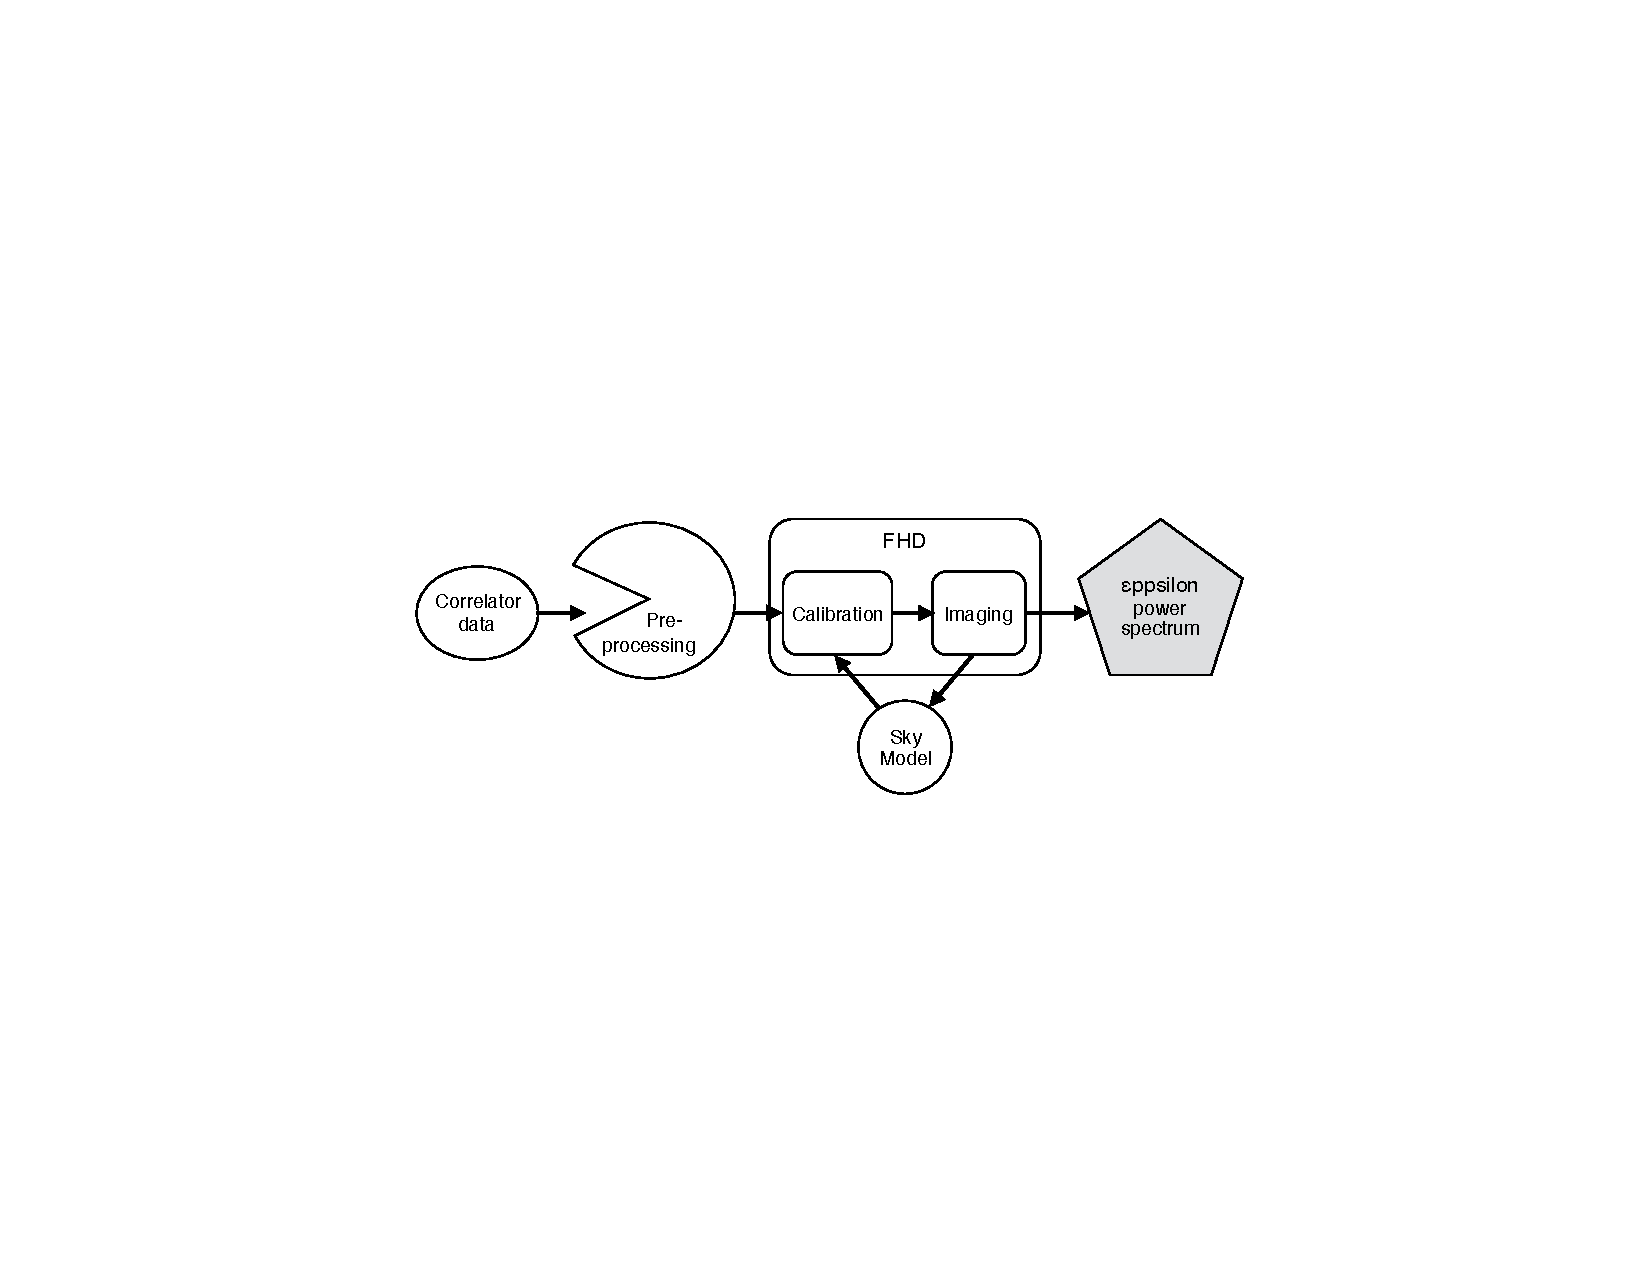
\includegraphics[width=\columnwidth]{pipe.pdf}
\caption[Pipeline diagram]{
Schematic of the analysis pipeline used in this work. The raw correlator data is 
preprocessed by performing RFI and other flagging. Then the data are calibrated and 
imaged using an iterative foreground modeling approach with the FHD package. Finally, a 
power spectrum is formed using the \eppsilon package.
\label{fig:pipe}
}
\end{center}
\end{figure}

\subsection{Preprocessing}\label{subsec:preprocessing}
The preprocessing step converts the data from the non-standard memory dump format 
from the correlator's GPUs to a standard UVFITS format \citep{Greisen:2012}, performs 
flagging, averages in time and freqeuncy, and writes to disk. For this step we use the 
\cotter package, which in turn calls the \texttt{AOFLAGGER}\footnote{\url{http://
aoflagger.sourceforge.net/}} to perform RFI flagging \citep{Offringa:2010}. 

Besides RFI, we manually flag data to remove three other effects. As mentioned in 
Section~\ref{sec:MWA}, the edges of the coarse bands contain high levels of aliasing from 
the filter applied in the digital receivers. We flag two 40 kHz channels on either side of the 
coarse band edges (total of four channels per coarse band edge). In principle the aliasing 
could be calibrated out and these channels could be recovered, but this is left for future 
work. Second, early data from the MWA also contained some instances where antennas 
were not pointed properly at the beginning of observations due to a beamformer error. This 
problem has since been resolved, but exists in our data. We therefore flag the first two 
seconds of each observation to avoid any potentially mis-pointed data. Finally, we flag the 
central fine channel of each coarse band because it corresponds to the DC mode of that 
sub-band and can easily float, washing out useful information.

In the final step of preprocessing, \cotter averages the data to 2 second, 80 kHz resolution 
and writes to disk. At this stage each snapshot is contained in a single UVFITS file, which 
serves as the base unit for calibration and imaging.


\subsection{Calibration and Imaging}\label{subsec:cal_imaging}
The next step in our pipeline is to calibrate the visibilities. As shown in Figure~\ref{fig:pipe}, 
a sky model is derived from our imaged data, which feeds back into the calibration. This is 
naturally an iterative process as the sky model is refined with improved calibration 
solutions. We will describe the sky model in detail in Section~\ref{sec:techniques}, but here 
we present the production mode of analysis after the model has been determined.

Calibration is accomplished within the FHD package in two steps. First we match the raw 
data to model visibilities formed using a realistic simulation of the array response to our 
foreground model. This step results in independent complex gains for each antenna, 
frequency channel, and polarization. In the second step we impose restrictions on these 
gains motivated by our understanding of the spectral response of the instrument. By 
reducing the number of free parameters in this step we increase our signal to noise on 
calibration solutions and avoid absorbing unmodeled confusion source flux into our gain 
solutions which has been shown to contaminate the EoR window \citep{Barry:2016}. 

In the first calibration step we allow our complex gains to account for any direction-
independent response on a per antenna, per frequency channel, per polarization basis. To 
define our gains in this way, we have made two simplifications. First we push all direction-
dependence of the antenna response into the model of the primary beam. FHD is capable 
of using separate models for each antenna, though this has not yet been implemented for 
the MWA due to lack of individual models. The second simplification is to ignore any cross 
terms between our different axes, for example a mutual coupling between two antennas. In 
principle these terms would introduce baseline dependent gains, rather than antenna 
dependent. The MWA has not yet seen evidence of these terms, and so we currently 
neglect them in our solutions.

Under these assumptions we can express the measured, uncalibrated visibility for an 
antenna pair $(i,j)$ as
\begin{equation}
V'_{ij}(\nu) \approx g_i(\nu)g^*_jV_{ij}(\nu),
\end{equation}
where $g_i(\nu)$ and $g_j(\nu)$ are the complex gains for antennas $i$ and $j$ 
respectively. Because we are treating polarizations independently, we allow the antenna 
subscript to run over both East-West (E-W) and North-South (N-S) polarizations.

FHD utilizes the StEFCal algorithm described in \citealt{Salvini:2014} to find the minimum 
$\chi^2$ estimate with respect to the complex gains. The result of this operation is 
estimated gains for every antenna, frequency channel, and polarization. However, with 
certain known properties of the antenna response we can reduce the number of free 
parameters in our solution. This takes us to the second step of calibration.

Our initial gain model included an amplitude bandpass common to all antennas, $B(\nu)$, 
and an antenna dependent low order polynomial in frequency. Mathematically we can 
express our restricted gain as
\begin{equation}\label{eq:cal1}
\hat{g}_i(\nu)=B(\nu)P_i(\nu),
\end{equation}
where the polynomial term can be further decomposed as
\begin{equation}
P_i(\nu) = (A_{i,0} + \nu A_{i,1} + \nu^2 A_{i,2})e^{i (\phi_{i,0} + \nu \phi_{i,1})}
\end{equation}
The coefficients $B(\nu)$, $A_{i,n}$, and $\phi_{i,n}$ are real quantities. This model allows 
us to capture arbitrary spectral response due to common antenna factors (such as the 
polyphase filter shapes or phased array response), as well as slowly varying antenna-
dependent deviations. We also found it necessary to include terms dependent on the 
beamformer to receiver cable length, which we will discuss in Subsection~\ref{sec:cables}.

Once all calibration terms are found, we complete the calibration by dividing the raw data by 
the gain estimates to produce calibrated visibilities. The entire calibration process is done 
for every snapshot of EoR data, providing both a two-minute resolution time dependence of 
calibration solutions, as well as model visibilities which are used for foreground subtraction 
and diagnostic purposes.

After calibration, we form snapshot image cubes (frequency mapping to line-of-sight 
direction). The visibilities are gridded using the primary beam as the gridding kernel, placing 
the data in the holographic frame, which has been shown to be the optimal frame for 
combining images in the sense that it preserves all information for parameter estimation 
\citep{Morales:2009,Bhatnagar:2008}. We use a simulation based beam model for MWA 
antennas developed by \citealt{Sutinjo:2015}. At this stage we also average in frequency by 
a factor of two by gridding pairs of frequency channels to the same $uv$ plane, resulting in 
a frequency resolution of 160 kHz. 

The gridded $uv$ data are then Fourier transformed to create sky-frame images. To avoid 
aliasing we image out 90$^\circ$ from phase center (gridding resolution of a half 
wavelength), and crop the image. We found that cropping the image based on beam value 
resulting in hard edges in integrated images from different snapshots having beams pointed 
in slightly different directions. To avoid the hard edges, we predetermine a set of HEALPix 
pixels to interpolate to, and use the same set for all snapshots on a given field. The final 
cropped field of view for this work is a 21$^\circ$ square centered at RA~$=0$ h, dec~
$=-27^\circ$. 

In principle the foregrounds could be subtracted from the data immediately after calibration, 
before gridding and imaging. However, for diagnostic reasons, we have found it beneficial to 
carry the model through the entire pipeline, and only subtract just before squaring to power 
spectrum units, allowing to form power spectra of the dirty, model, and residual data.

FHD provides all inputs needed for the \eppsilon package, which include weights cubes (for 
proper accumulation of data), variance cubes (for error propagation), and even/odd 
interleaved data cubes (for an unbiased estimator and a direct measurement of the noise). 
We also retain both East-West and North-South polarizations. At this time we can remap 
our coordinates to cosmological units according to the relationships given in 
\citealt{Morales:2004}, where angular and frequency units $(\theta_x,\theta_y,f)$ map to 
cosmological distance units $(r_x,r_y,r_z)$. Often $r_z$ is referred to as the line of sight 
dimension, and denoted as $r_{||}$. Similarly, $(r_x,r_y)$ is the plane perpendicular to the 
line of sight and is denoted as $\mathbf{r_{\perp}}$.

\subsection{Power Spectra}
In the final steps of our pipeline we integrate the snapshot image cubes, and calculate a 
power spectrum estimate. Though the integration step is formally an imaging component, 
we conceptually group it with the power spectrum step. This is because all steps of the 
pipeline up to here have been performed on a per-snapshot basis (no communication 
between snapshots beyond foreground modeling), and the integration step can be used to 
select subsets of data for diagnosing power spectrum artifacts. The images produced by 
FHD are in the holographic frame, which is already properly weighted for combining 
images, so the integration is simply adding the cubes together, and propagating the 
weights.

The \eppsilon package performs a discrete Fourier transform (DFT) on each $r_{||}$ slice of 
the integrated HEALPix cube, forming a cube in $(\mathbf{k}_{\perp},r_{||})$, where $
\mathbf{k}_{\perp}$ represents the cosmological wavenumber in the plane perpendicular to 
our line of sight, and $r_{||}$ is the distance to the observed redshift slice along the line of 
sight. The Fourier transform along the $r_{||}$ dimension is treated separately due to 
incomplete $uv$ sampling and flagged frequency channels, which leads to structure in the 
frequency sampling along any given $k_{\perp}$ pixel. We thus adopt the Lomb-Scargle 
least-squares method to determine the orthogonal eigenfunctions given our sampling 
function and estimating the total power in each $k_{||}$ mode \citep{Scargle:1982}. In 
addition, because the spectrally smooth foregrounds contain vastly more power than the 
expected EoR signal, we apply a Blackman-Harris window function prior to the $r_{||}$ to 
$k_{||}$ transform. This has the effect of trading off lower effective bandwidth for higher 
dynamic range.

After squaring and dividing by our observation window function \citep{Bowman:2006}, we 
arrive in three dimensional power spectrum space. We use the even/odd interleaved cubes 
to form a signal (odd plus even) and noise (odd minus even) power spectrum, which we 
subtract from one another to form an unbiased estimate of our signal power. This is 
mathematically equivalent to cross multiplying the even and odd cubes. The three 
dimensional power spectrum cube can next be averaged in annuli to form two dimensional 
power spectra, or spherical shells to form one dimensional power spectra where we will 
ultimately constrain the EoR.

\begin{figure}
\begin{center}
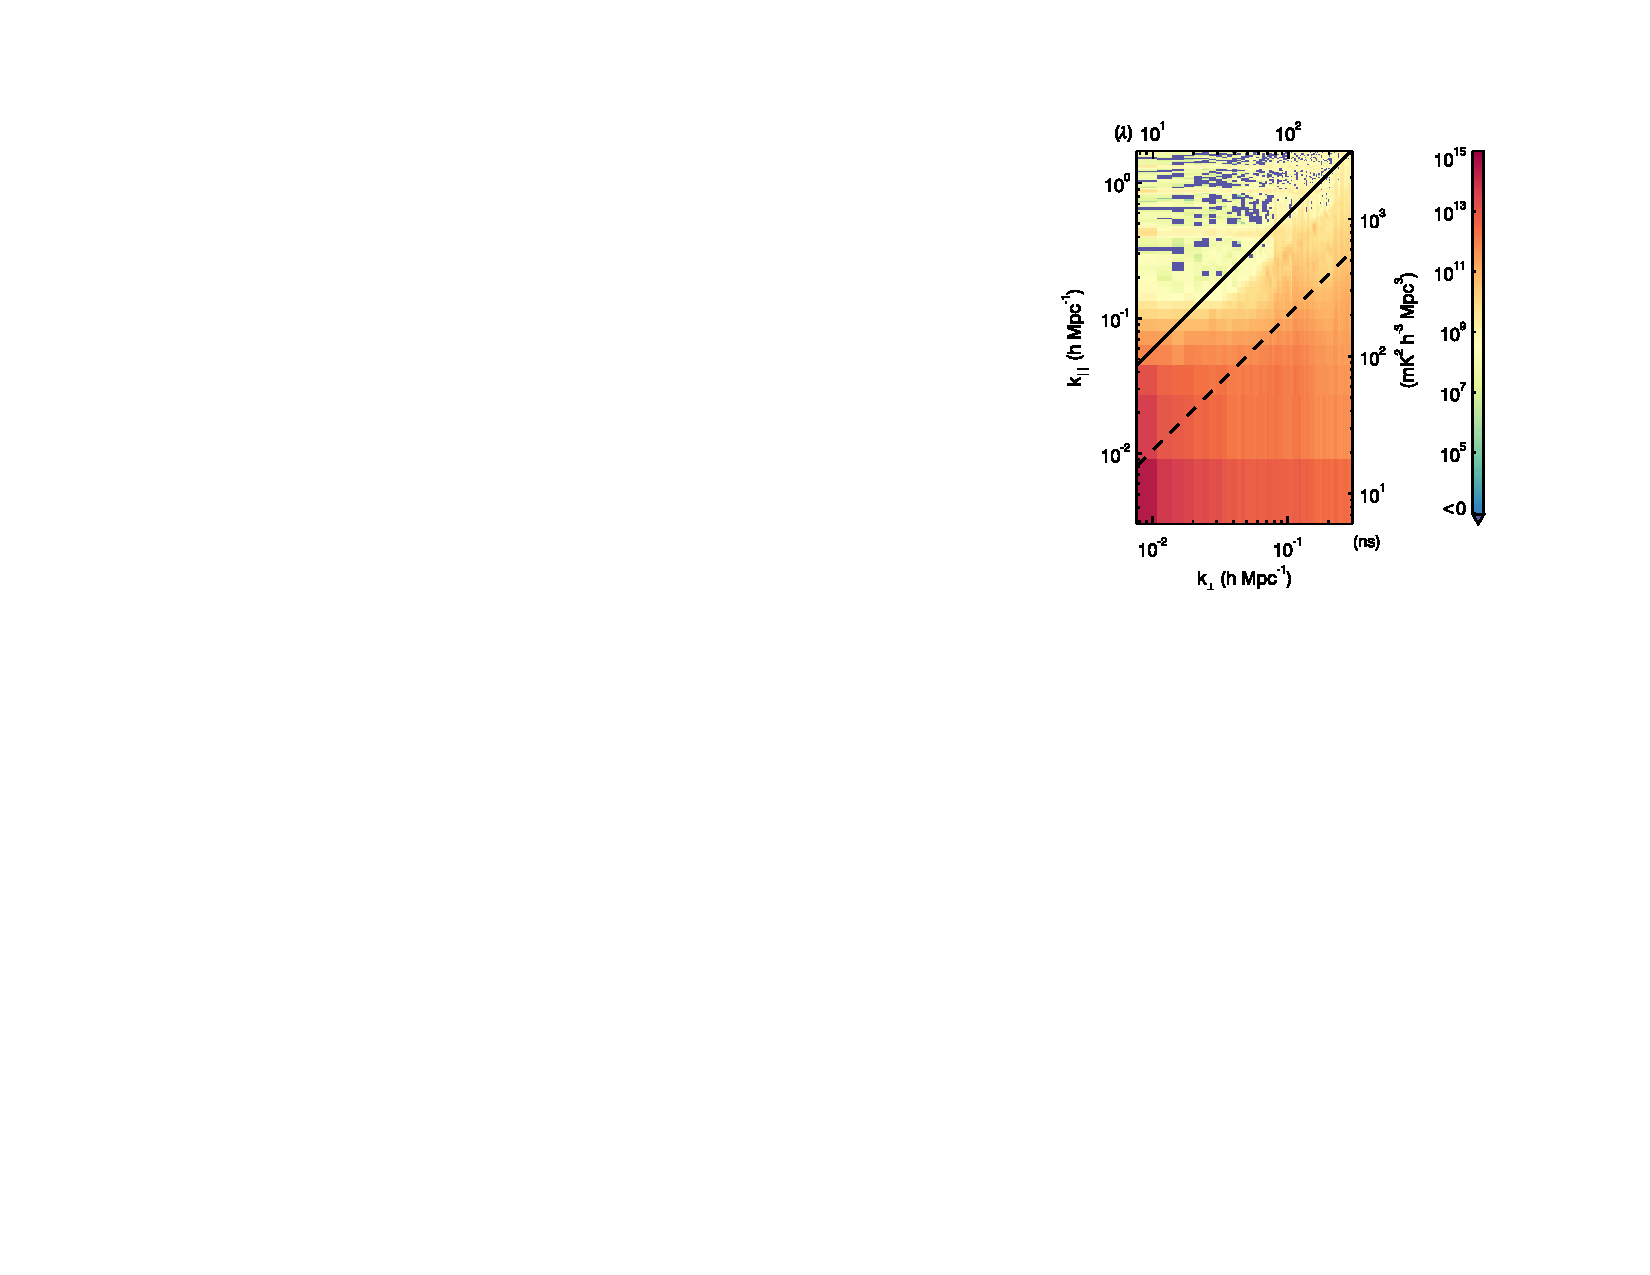
\includegraphics[width=.9\columnwidth]{example_ps.pdf}
\caption{
An example two dimensional, E-W polarization residual power spectrum formed using the 
three hour golden data set. The foreground wedge dominates the region below the solid 
black horizon line, while regions above are mostly noise-like with the exception of horizontal 
coarse band harmonic lines. 
\label{fig:example_ps}
}
\end{center}
\end{figure}

An example two dimensional residual power spectrum formed from the three hour golden 
data set is shown in Figure~\ref{fig:example_ps}. The bulk of the residual power is in the 
so-called foreground ``wedge", indicated with the diagonal black lines where the solid line 
corresponds to sky emission at the horizon, and the dashed lines corresponds to emission 
at the edge of the MWA field of view. Above the wedge we see horizontal lines of 
contamination due to the periodic frequency sampling function. These lines are often 
referred to as the coarse band harmonics. We see vertical streaks at high $k_{||}$ and high 
$k_{\perp}$. These are due to sparse $uv$ sampling beyond the dense core of the MWA 
(starting $\sim70\lambda$), and the foreground power getting thrown to high spectral 
modes. Between the coarse band lines and to the left of the vertical streaks we see regions 
which contain both positive and negative (indicated by blue on the color bar) pixels. These 
regions are where we have successfully isolated the foregrounds and retained a noise-like 
EoR window in the three hour integration.

\section{Novel Analysis Methods}\label{sec:techniques}
\textcolor{red}{Needs a better section title}

The two dimensional power spectrum is a useful figure of merit (FoM) as we improve and 
refine our analysis pipeline. Foregrounds and systematics often manifest with characteristic 
shapes in this space, enabling us to diagnose problems and quantify improvements 
\citep{Morales:2012}. We use the MWA 3 hour ``golden'' data set from August 23, 2013, to 
repeatedly form power spectra to test and refine our analysis. While an exhaustive catalog 
of these improvements would be unsuited for this article (and likely bore the reader), we 
demonstrate the utility of the 2D power spectrum as a FoM with a few key techniques we 
have employed in our analysis. 

\subsection{Cable Dependent Calibration}\label{sec:cables}

Early in our analysis it became apparent that the bandpass of each MWA antenna requires 
more free parameters than those described in equation~\ref{eq:cal1}. In particular, differing 
beamformer to receiver cables lead to different bandpass shapes due to signal attenuation. 
We therefore allow the amplitude bandpass factor to depend on cable length, $B_{\alpha}
(\nu)$, where $\alpha$ denotes the cable type.\footnote{For logistical purposes the 
beamformer to receiver cables were installed in six set lengths. Cables of length 90, 150, 
and 230 meters are RG-6, while 320, 400, and 524 meter cables are LMR400-75.}

The top panel of Figure~\ref{fig:cables} shows a 2D power spectrum using the gain model 
described so far. Three of the horizontal lines in the EoR window can be attributed to the 
coarse band gaps, as they reside at the harmonics expected for 1.28~MHz periodic 
sampling. But the sampling cannot account for the fourth line, highlighted by the arrow. The 
corresponding delay time of the line, $\tau \approx 1.23$~$\mu$s, corresponds almost 
exactly to twice the signal travel time through the 150 meter cables (with velocity 0.81c). We 
therefore introduced a reflection term into our gain model, which allows our restricted gains 
to account for the interference of the incident signal with a round-trip reflected signal in the 
cable. The full gain model is expressed as
\begin{equation}\label{eq:cal2}
\hat{g}_i(\nu)=B_{\alpha}(\nu)\left(P_i(\nu)+R_i(\nu)\right),
\end{equation}
where the reflection term can be further decomposed as
\begin{equation}
R_i(\nu) = R_{i,0} e^{-2\pi i \tau_{i} \nu}.
\end{equation}
The reflection coefficient, $R_{i,0}$ is allowed to be complex, while the reflection delay, 
$\tau_i$ is real. After fitting for all other parameters, we fit for the reflection mode. This is 
done for antennas with suspected reflections, the most offensive of which is seen in the 
antennas with cables of 150 meters. Because the cables were not cut at exact lengths 
(variations on order tens of centimeters), we solve for both the reflection coefficient and 
delay by performing a direct Fourier transform to a highly over resolved delay grid and 
selecting the mode where the reflection amplitude is largest. 

\begin{figure}
\begin{center}
\subfigure{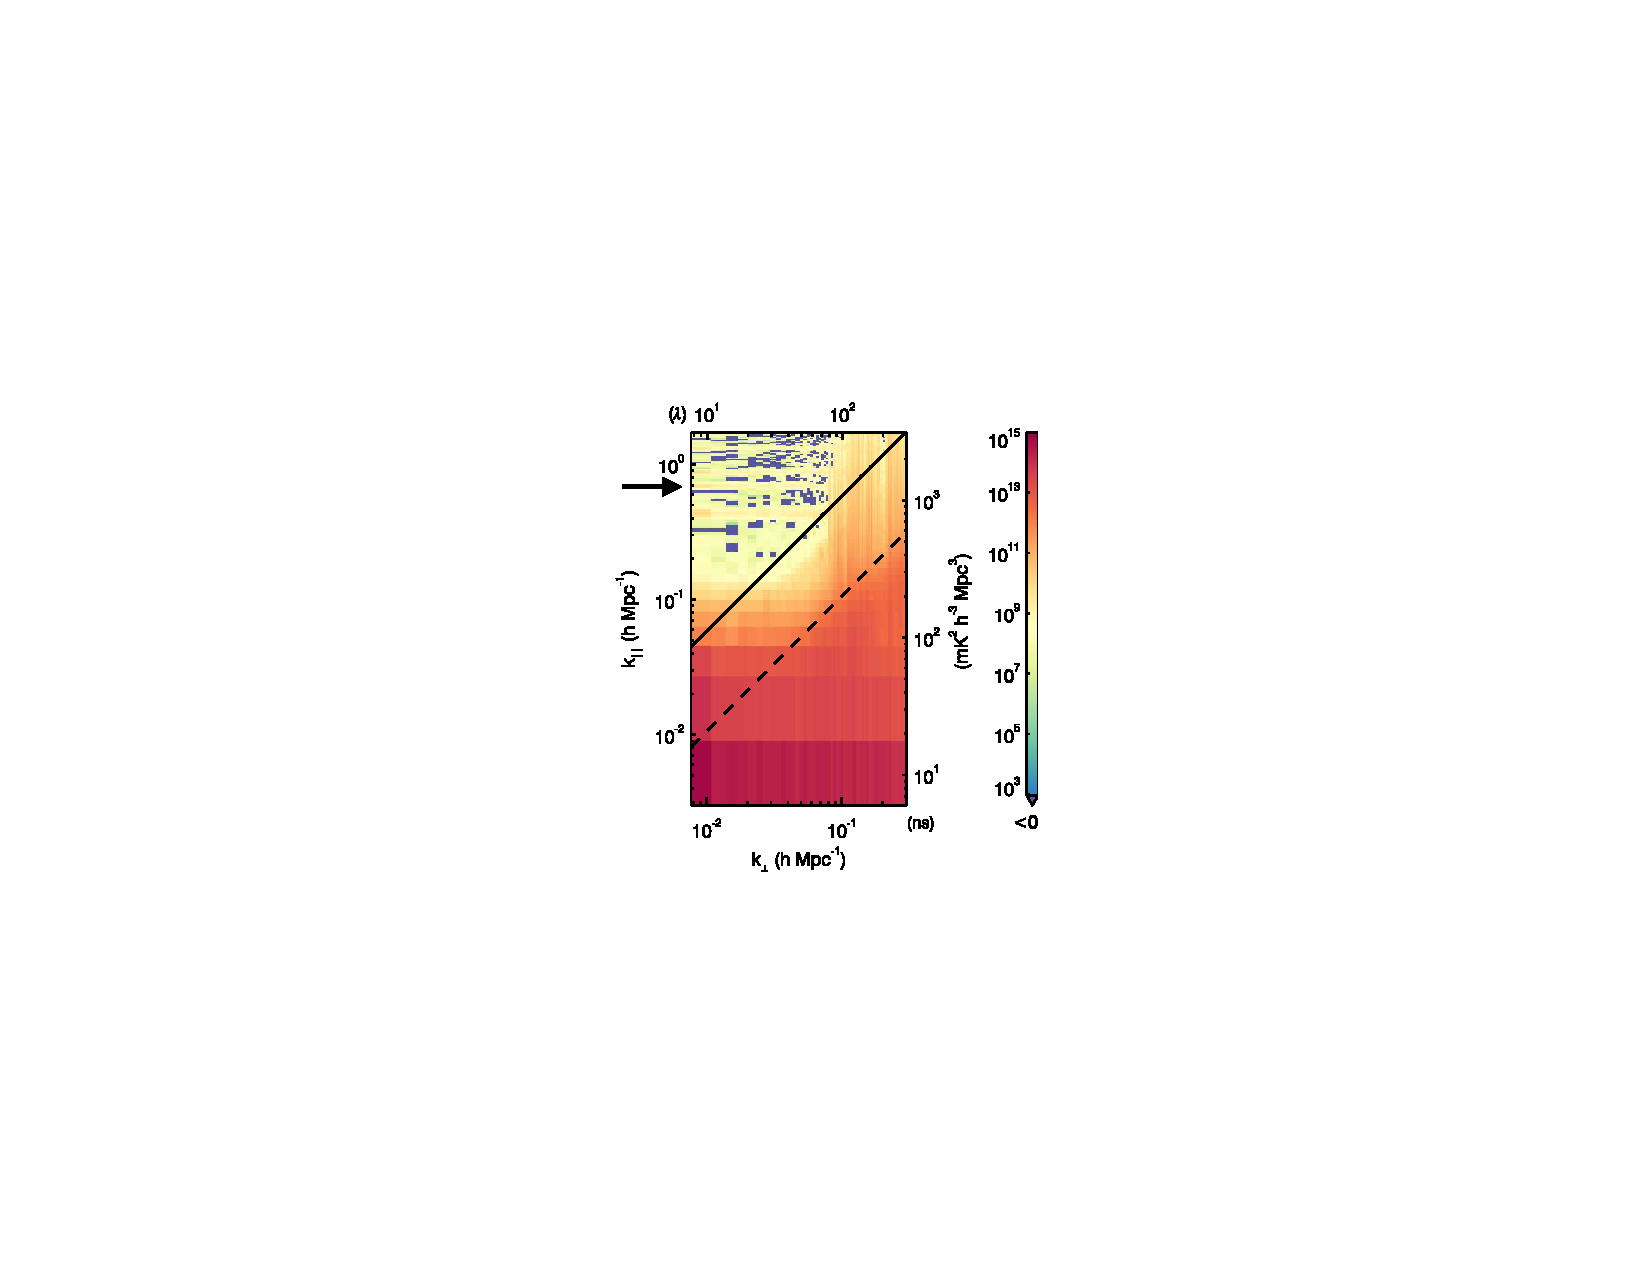
\includegraphics[width=.9\columnwidth]{fourth_line_pre.pdf}}
~
\subfigure{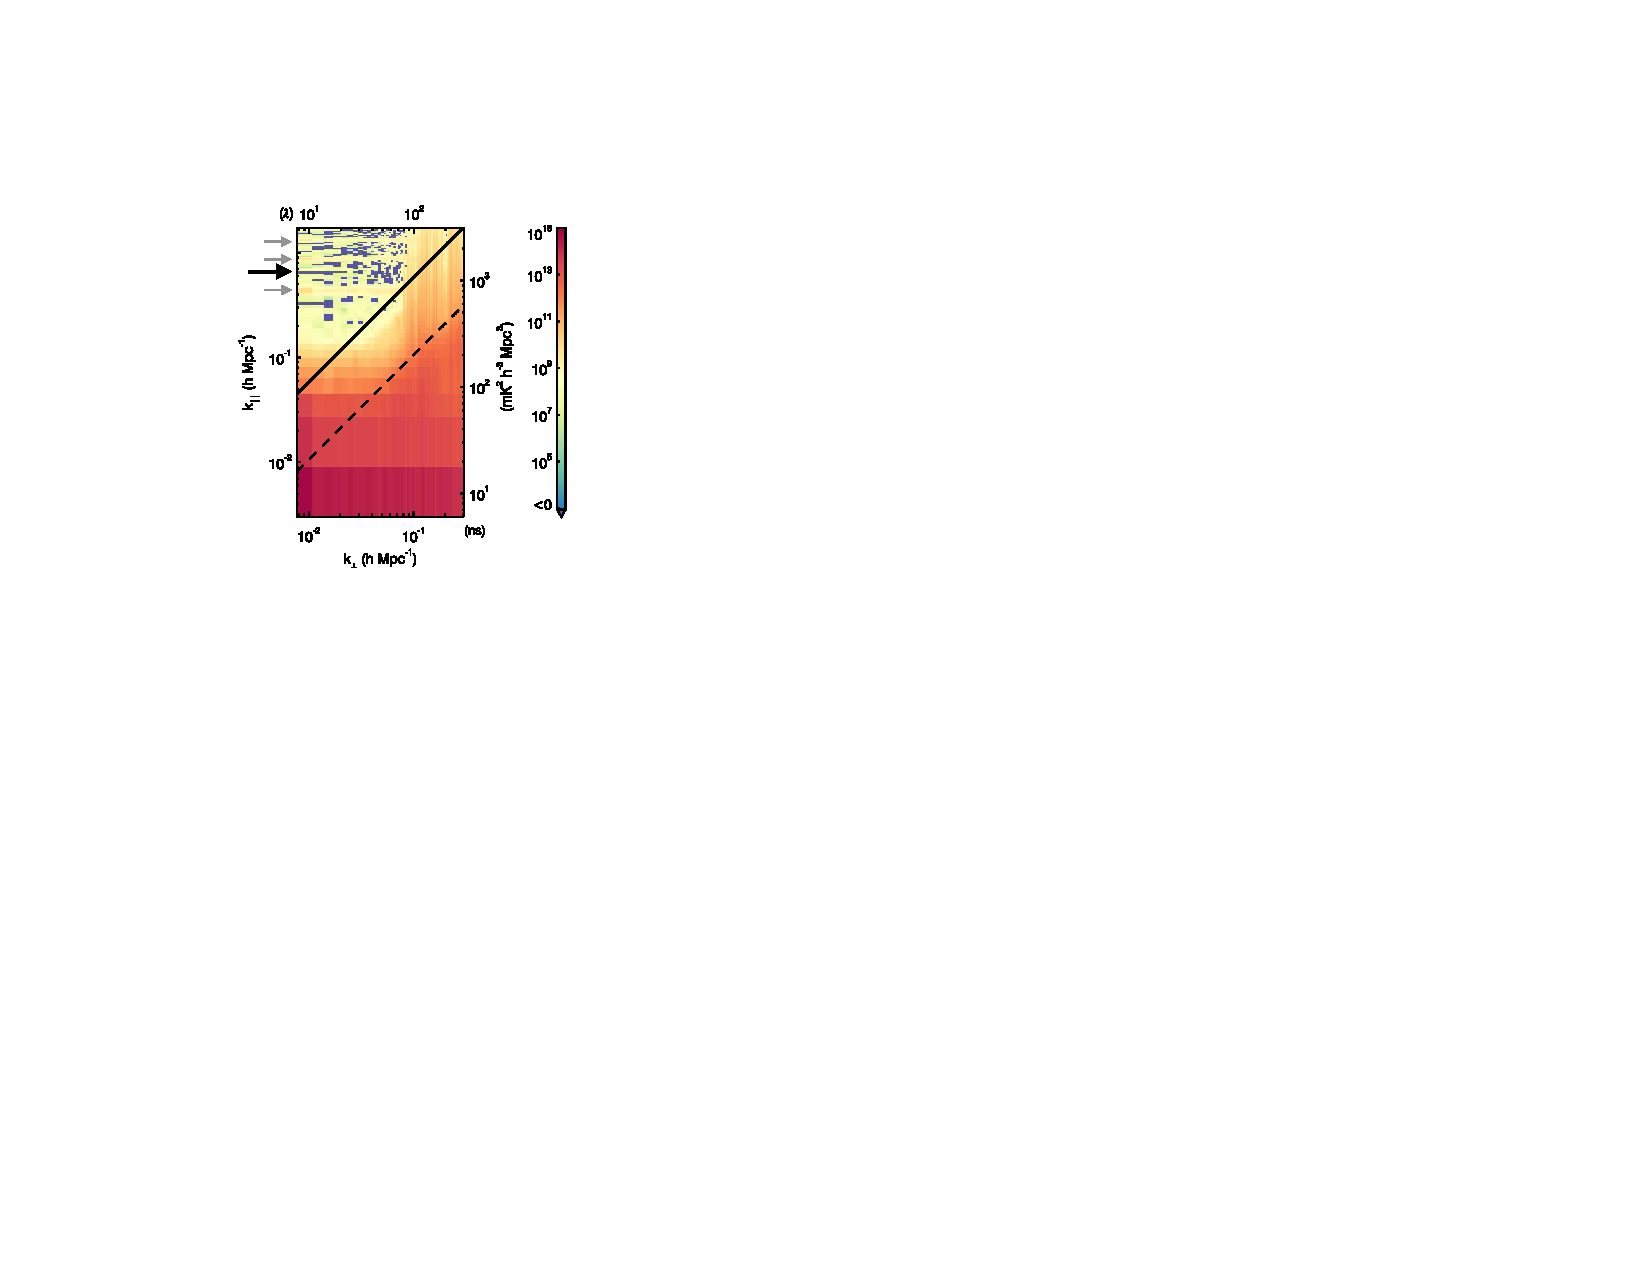
\includegraphics[width=.9\columnwidth]{fourth_line_post.pdf}}
\caption{
\emph{Top:} Single polarization dirty power spectrum formed from the golden data set, 
before implementing cable reflection fitting into the calibration loop. The black arrow points 
to a horizontal band at $k_{||} \approx 0.6$~h~Mpc$^{-1}$, which cannot be accounted for 
by the coarse bands. \emph{Bottom:} After we implement the cable reflection fitting in our 
calibration solutions, we see the reflection line disappears.
\label{fig:cables}
}
\end{center}
\end{figure}

The resulting 2D power spectrum after fitting for cable reflections is shown in the bottom 
panel of Figure~\ref{fig:cables}, where the reflection line is suppressed below the noise 
level. This example demonstrates the power of the 2D power spectrum as a figure of merit. 
The power in the reflection line was about five orders of magnitude below the foregrounds, 
making it very difficult to detect in image-based metrics. However the power spectrum is 
specifically designed to be sensitive to low-level spectral structure, and using the two 
dimensional spectrum allows us to identify the ``shape'' of contamination, enabling a 
precise diagnosis.

\subsection{Gridding Kernel Resolution}
A similar, low level effect which had the potential to contaminate the EoR window is shown 
in Figure~\ref{fig:beam_res}. The spectra shown are the \emph{model} spectra -- calculated 
by propagating the sky model visibilities through the entire pipeline. Despite our foreground 
model not containing spectral structure, the EoR window in the left panel seems to have a 
floor at a level $\sim 10^7$~mK$^2$~h$^{-3}$~Mpc$^3$, comparable to predicted EoR 
signals. In addition there is a faint line in the upper-left of the plot which has the same slope 
as the wedge, but seems to originate far beyond the horizon.

\begin{figure}
\begin{center}
\subfigure{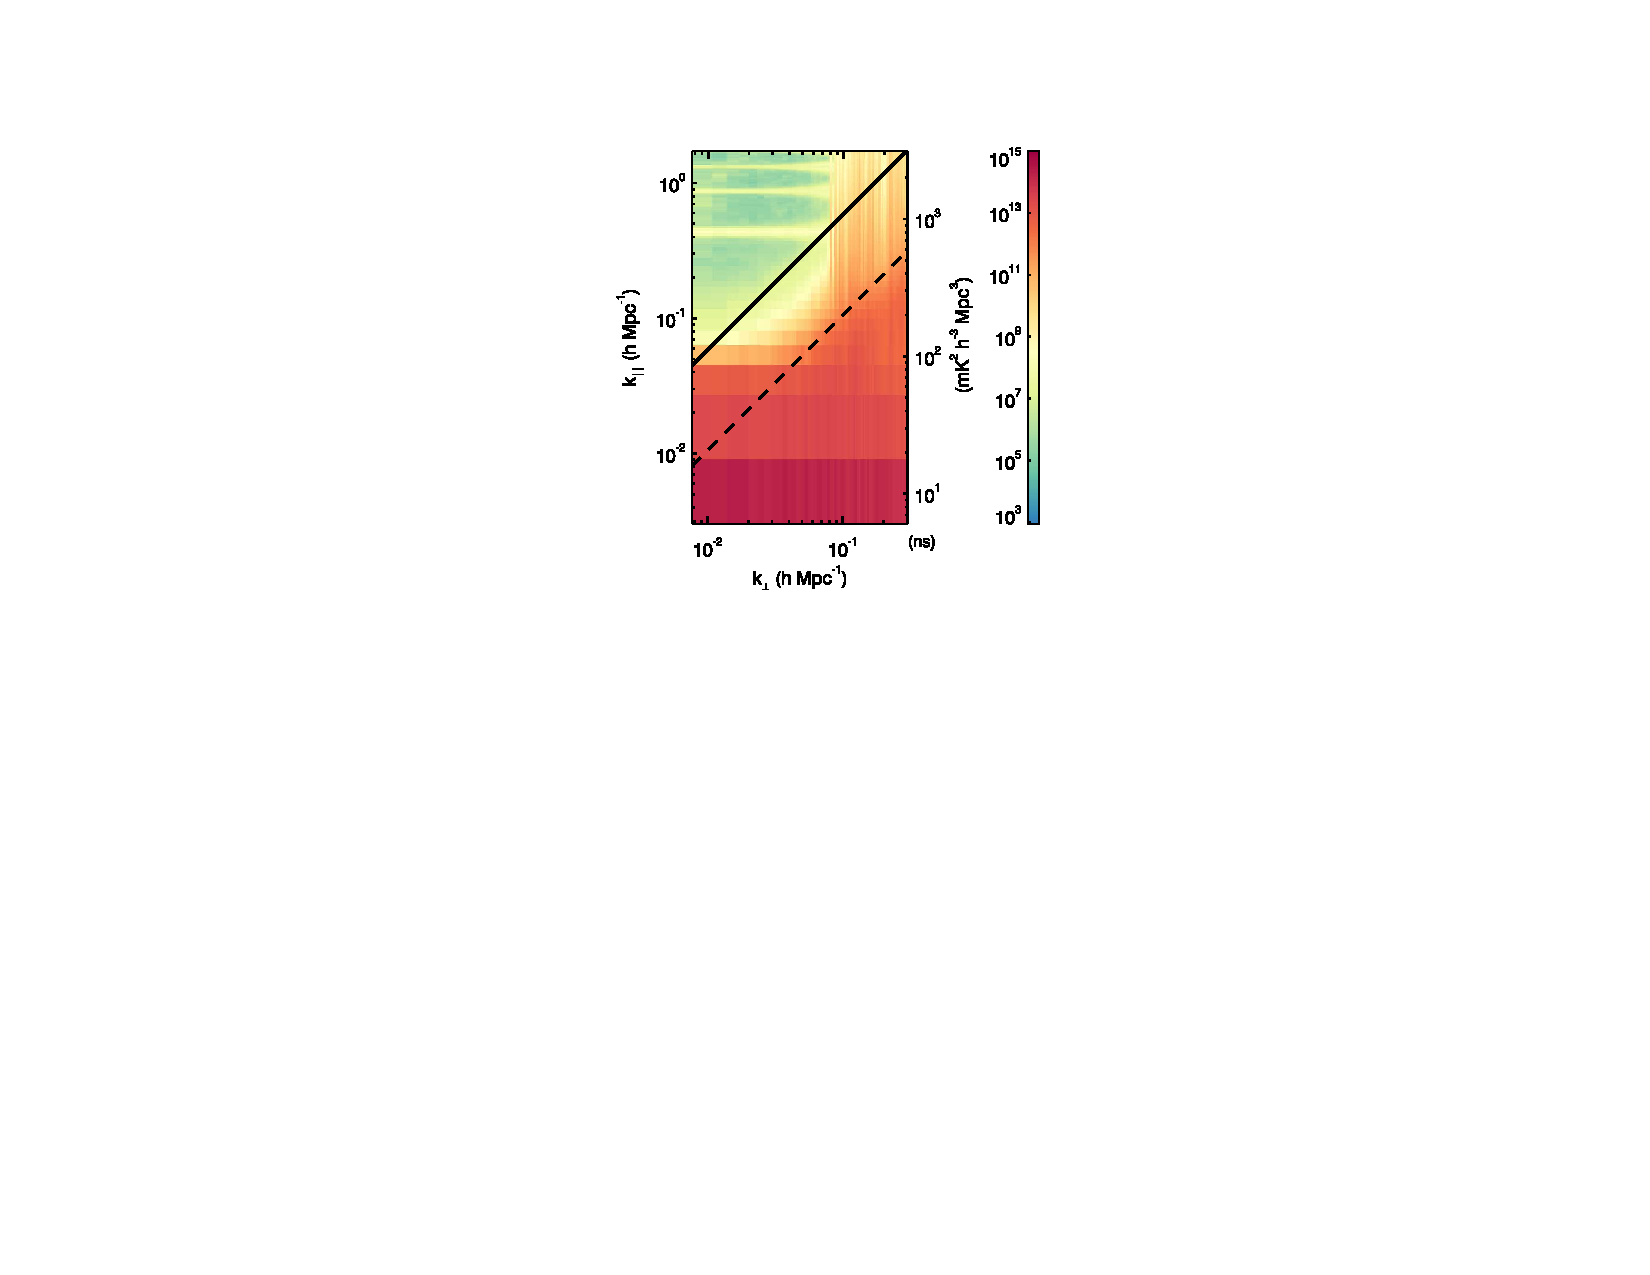
\includegraphics[width=.9\columnwidth]{before_beam_resolution_golden.pdf}}
~
\subfigure{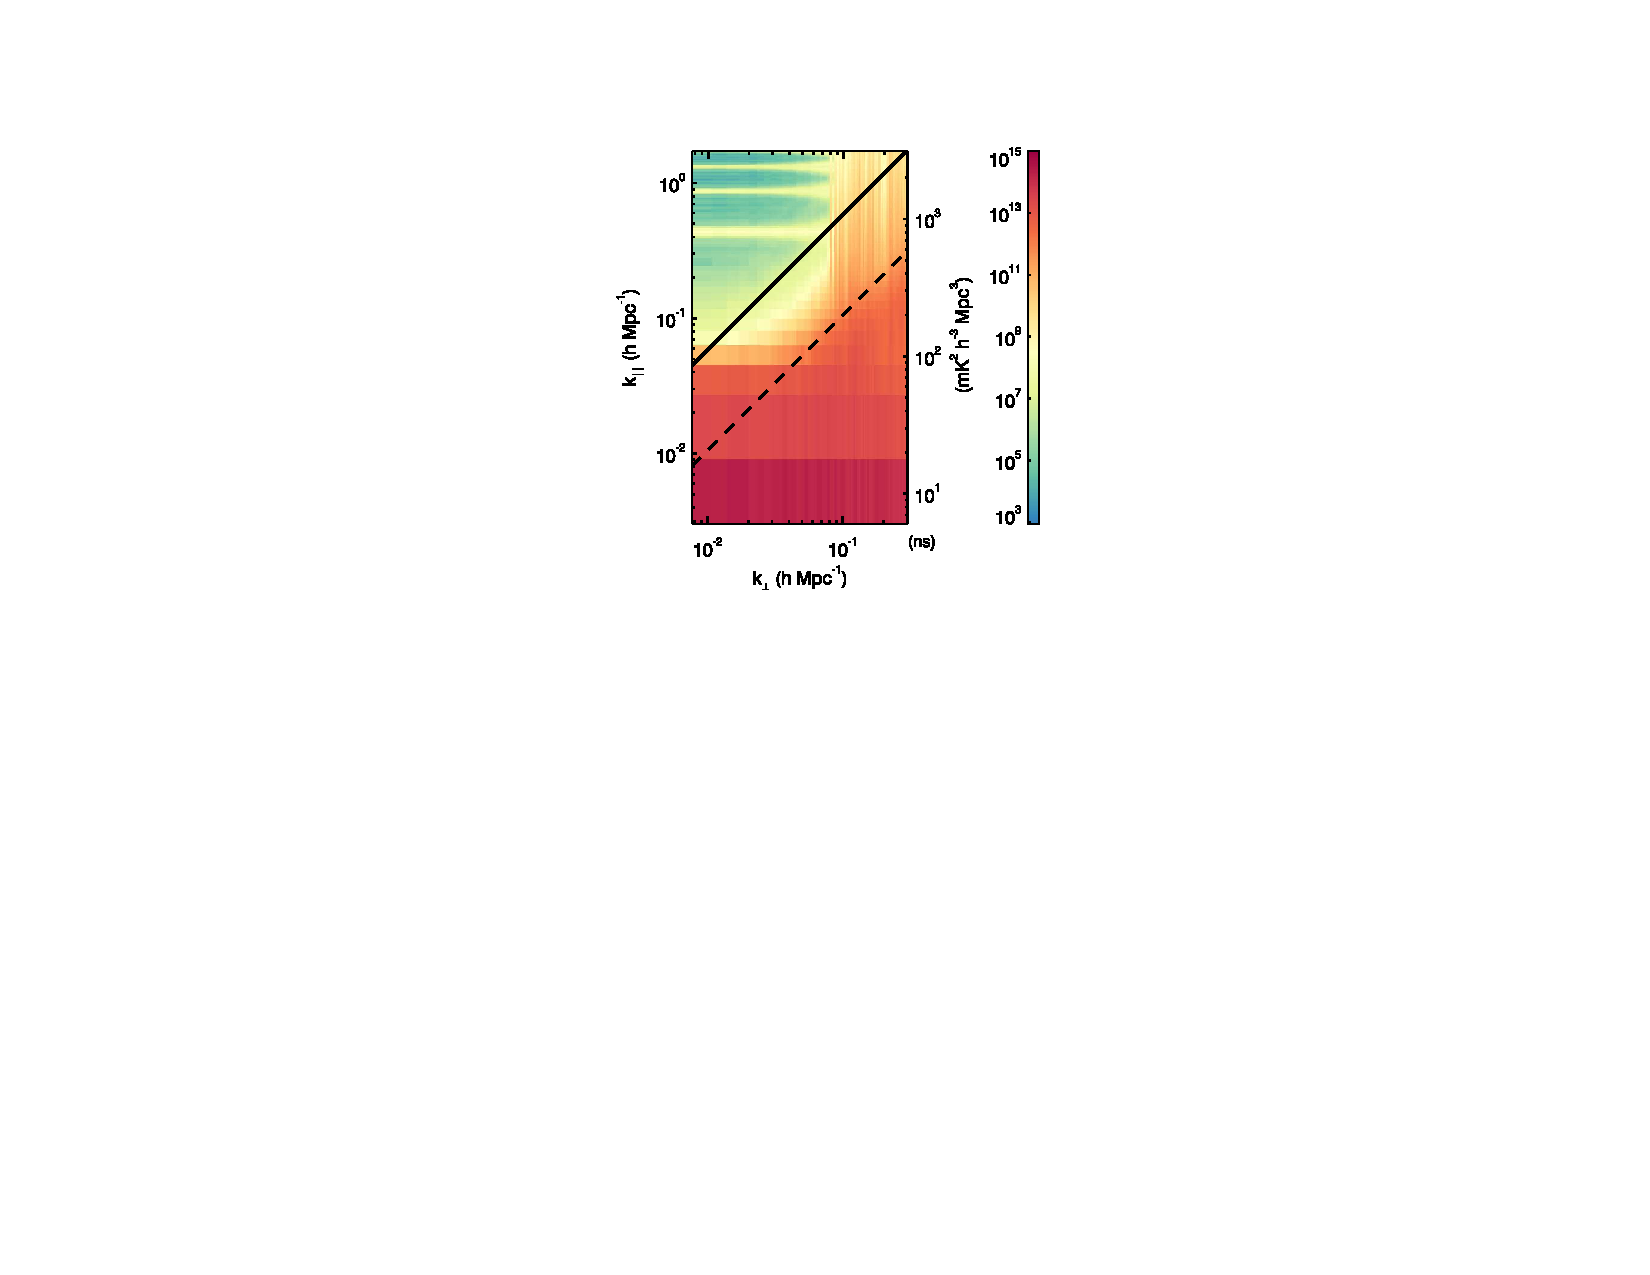
\includegraphics[width=.9\columnwidth]{after_beam_resolution_golden.pdf}}
\caption{
\emph{Top:} Single polarization model power spectrum demonstrating the contamination in 
the EoR window when using insufficient gridding kernel resolution. The window has a floor 
comparable to an expected EoR signal, and a faint super-horizon line appears at high 
$k_{||}$. \emph{Bottom:} Model power spectrum after increasing the gridding kernel 
resolution from 0.04 wavelengths to 0.007 wavelengths. The floor is now far below the 
expected EoR signal level. 
\label{fig:beam_res}
}
\end{center}
\end{figure}

The source of this floor and super-horizon line ended up being the resolution at which we 
formed the gridding kernel when gridding visibilities. In the interest of computational speed 
and efficiency, the kernel is pre-calculated at a high resolution, then a nearest neighbor 
lookup table is used to approximate the beam values at discrete pixels. The kernel 
resolution used in the top panel of Figure~\ref{fig:beam_res} was 0.04 wavelengths -- much 
smaller than the half wavelength grid corresponding to horizon to horizon imaging. 
However, as a baseline migrates in $\emph{uv}$ coordinates across frequencies, it 
undergoes discrete steps between kernel values used. This effectively results in small 
baseline position errors which shift periodically in frequency, resulting in power being thrown 
up into the window and a relatively strong harmonic at the frequency of the shifting (the faint 
line in the upper left of the window). While we illustrate this effect with a model power 
spectrum, the same problem exists in the data, but is below the noise levels at three hours 
of integration.

We resolved this issue by increasing the resolution at which we form the kernel. While the 
most accurate answer is to model at infinite resolution, it is not feasible to do so 
computationally. Instead we chose a resolution at which the effect no longer materially 
impacts the power spectrum. With experimentation we found a kernel resolution of 0.007 
wavelengths was sufficient. The resulting model power spectrum is shown in the bottom 
panel of Figure~\ref{fig:beam_res}. The contamination within the EoR window now drops 
significantly below the predicted cosmological signal levels.

\subsection{Improving Point Source Model}

Our pipeline uses two modes of FHD -- the full deconvolution mode to identify point sources 
and build a catalog, and a production mode where we calibrate using the sky model and 
subtract it from the data without further fitting. Because full deconvolution on every 
observation from the MWA is computationally not feasible, we currently restrict ourselves to 
the golden data set to build our model. The process of building the catalog is presented in 
P.~A.~Carroll et al. 2016 (in review). They applied machine learning classification methods 
to select reliable detections from the full deconvolution FHD mode, culminating in the KGS 
catalog. The work here uses an early iteration of the KGS catalog that was available at the 
time of analysis.

It has been shown that subtracting a foreground model strictly within the main lobe of the 
primary beam will not be sufficient to suppress the power spectrum wedge and unlock the 
EoR window \citep{Pober:2016, Thyagarajan:2015, Thyagarajan:2015b}. In principle we 
can repeat the model building described above using additional MWA observations pointed 
away from our field of interest. But until that work is complete we supplement the extent of 
our point source model using additional catalogs. We accomplish this through a hierarchical 
catalog pulling from our early KGS catalog, the MWA Commissioning Survey\footnote{The 
more complete GLEAM Survey \citep[][Hurley-Walker et al., in collaboration review]
{Wayth:2015} was not available at the time of analysis.} \citep[MWACS, ][]
{Hurley-Walker:2014}, Culgoora \citep{Slee:1977}, and the Molonglo Reference Catalog 
\citep[MRC, ][]{Large:1981}. Source fluxes are prioritized in this order based on our 
confidence in their predicted flux at 182 MHz. We first cluster the source lists to avoid 
redundant sources, using a 3.5 arcmin neighborhood radius, then select the flux from the 
highest priority catalog. Spectral indices were obtained from the MWACS and Culgoora 
catalogs when available, otherwise a two-point spectral index was estimated for Culgoora-
MRC matches or MRC-SUMSS matches. All other sources were given a spectral index of 
$-0.8$. The spectral index was used to extrapolate the flux from the catalog frequency to 
182 MHz, but a uniform spectral index of $-0.8$ is used within our band when forming 
model visibilities for calibration and foreground subtraction.

The resulting hierarchical catalog is shown in Figure~\ref{fig:master_catalog}. The EoR0 
field corresponds to the red FHD source patch. All sources above the horizon and within a 
primary beam value greater than 1\% maximum (including sidelobes) are included in both 
our calibration and foreground subtraction models.  

\begin{figure*}
\begin{center}
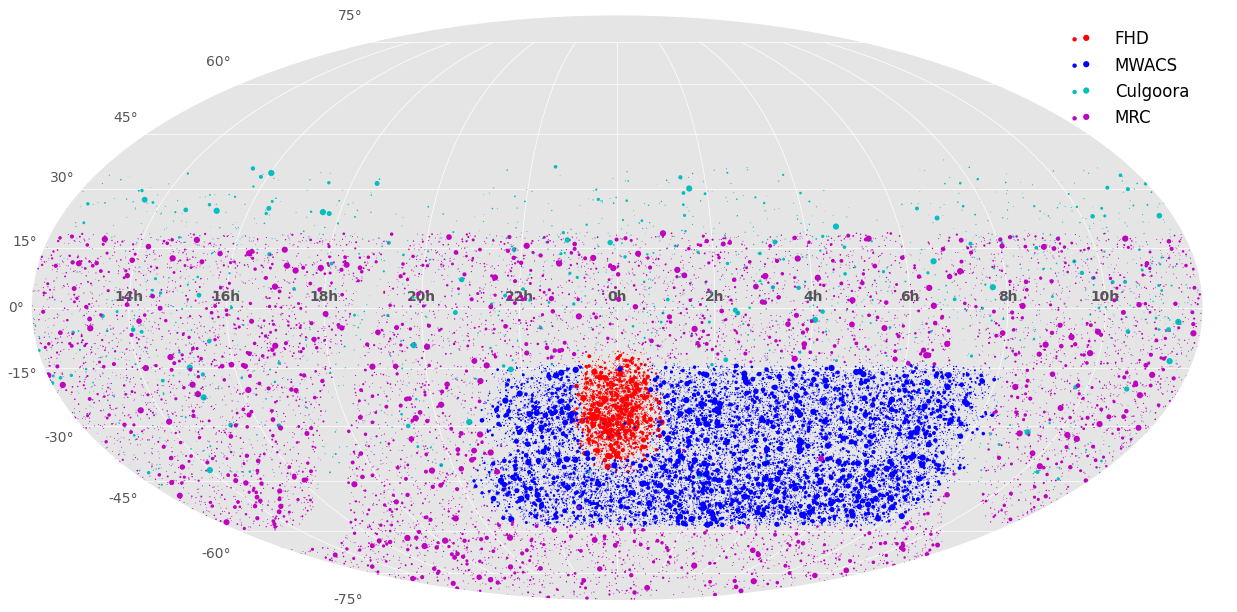
\includegraphics[width=\textwidth]{master_catalog.png}
\caption{
Hierarchical catalog used for foreground subtraction. This catalog combines the source lists 
from our own FHD catalog, the MWACS catalog, Culgoora sources, and the MRC, 
prioritizing in that order. The EoR0 field corresponds to the red FHD patch, while we use the 
other catalogs to fill in the sidelobes of the MWA. The size of each dot is proportional to the 
182~MHz flux of the source, clipped at 20~Jy.
\label{fig:master_catalog}
}
\end{center}
\end{figure*}

To show the effect our hierarchical catalog has on the power spectrum figure of merit, we 
ran our entire analysis pipeline on the golden data set with two foreground models -- first 
with only the MWACS catalog, and again with the full hierarchical catalog. We then 
compare the resulting 2D power spectra to inspect whether the new catalog results in more 
accurate calibration and foreground subtraction.

Because we use the input foreground model to calibrate our visibilities, the gain estimates 
for our two runs differed. In particular we saw the overall flux scale of the calibrated 
visibilities was higher when using the full hierarchical catalog. In order to put both residual 
2D power spectra onto the same scale for comparison, we first divide each pixel by the 
corresponding dirty power spectrum pixel, then subtract to arrive at a ratio difference. 
\begin{equation}\label{eq:diff_ratio}
\mathtt{ratio\;difference = \frac{residual_1}{dirty_1} - \frac{residual_2}{dirty_2}}
\end{equation}
Here we use subscript 1 to represent the MWACS catalog spectra, and 2 for the 
hierarchical catalog spectra. The ratio difference is shown in Figure~\ref{fig:mwacs_ratio}. 
The entire wedge being positive (blue) demonstrates that using the new catalog resulted in 
successfully subtracting higher fractional power. Not only does this indicate we subtract 
more power, but it also confirms that our calibrated data is more closely matched to the 
model, meaning that the higher flux scale seen in the left panel of Figure~
\ref{fig:mwacs_diff}, and our calibration solutions in general, are more accurate.

\begin{figure}
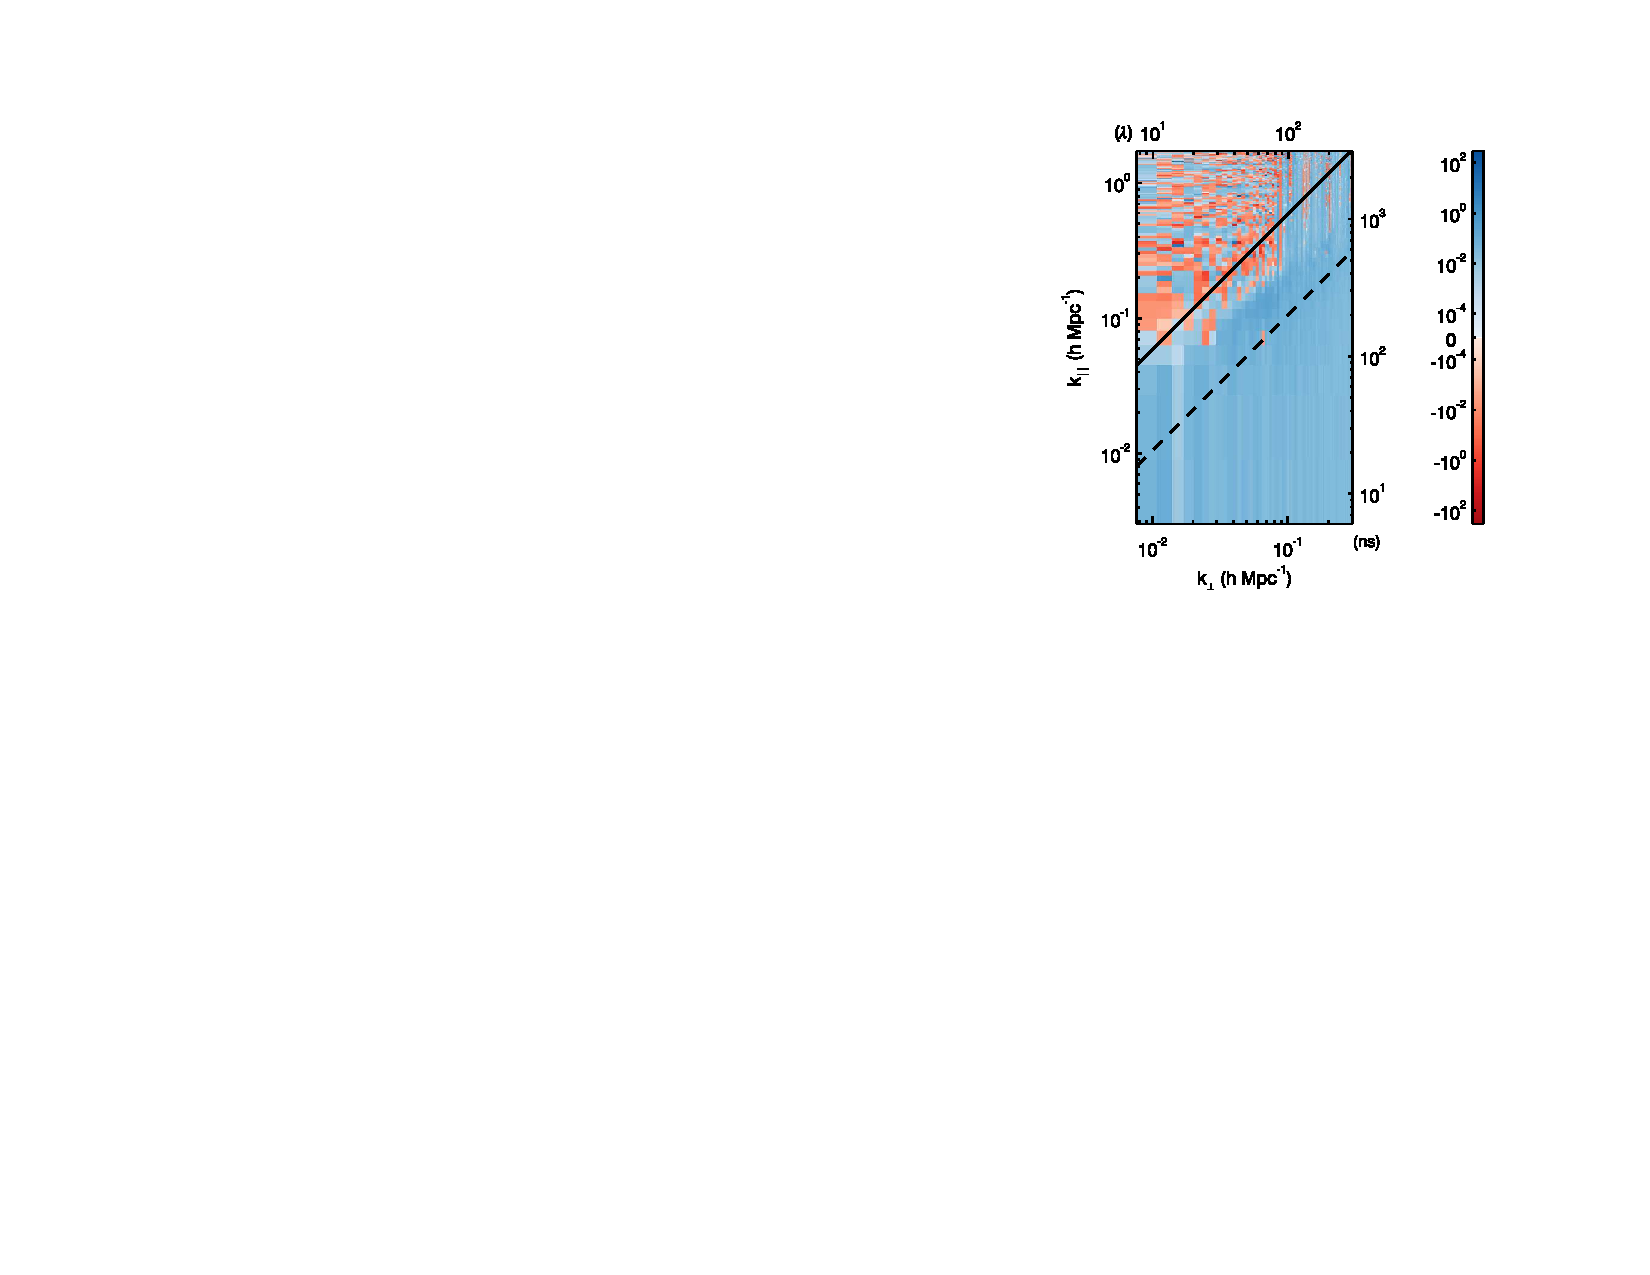
\includegraphics[width=\columnwidth]{mwacs_ratio.pdf}
\caption{Power spectrum ratio difference, according to equation~\ref{eq:diff_ratio}. This 
metric shows the difference in the fractional E-W residual 2D power spectrum, comparing 
the MWACS catalog and our hierarchical catalog. By dividing the residual spectrum by the 
corresponding dirty spectrum before subtracting we remove the effect of the overall flux 
scale change due to differing calibration solutions. We see that the wedge is completely 
positive (higher fractional residual when using the MWACS catalog), confirming that the 
hierarchical catalog subtracts more power from the data. This also reassures that the 
calibration using the new catalog is more accurate. 
\label{fig:mwacs_ratio}
}
\end{figure}

\subsection{Diffuse Foreground Model Subtraction}

In addition to a point source foreground model, we also introduce a diffuse emission model 
within the primary field of view of the MWA. Though the EoR0 field was chosen to be 
relatively devoid of galactic emission, we find this diffuse structure still highly contaminating 
due to the very high sensitivity of the MWA at large scales. For computational purposes we 
have divided the galactic emission into two regimes -- the faint clouds in our main lobe, and 
the bright plane and other structures in the sidelobes. While the latter has been studied by 
many people and a Global Sky Model (GSM) is readily available 
\citep{deOliveira-Costa:2008}, the computational obstacle of simulating the instrument 
response to a full sky diffuse model is yet prohibitive, though under active pursuit 
\citep{Thyagarajan:2015}. We instead focus here on diffuse structure within the primary field 
and leave the full-sky model to future iterations of analysis.

This first iteration of modeling the diffuse structure within our primary field was done by 
simply using output point-source subtracted residual images of FHD from the three hour 
golden data set. We combine the images from three hours to leverage the rotation of the 
earth to improve the point spread function (PSF) of the instrument. This integrating of 
images is done in a uniformly weighted frame to minimize the effect of double instrument 
convolution (once when the data is taken, again when we use the output as a model). We 
then form a pseudo Stokes I image by adding beam-weighted East-West and North-South 
polarizations. We also integrate in frequency to form a single continuum image for our 
model. By forcing our model to contain no spectral structure we mitigate the risk of 
subtracting cosmological signal. Future iterations of this model will contain a spectral index 
and multiple polarization components.

Ultimately we need model visibilities to subtract from our data. However, rather than storing 
a model for all observations (different pointings and phase centers), we find it most simple 
to treat the model as a single HEALPix image which can be used to create model visibilities 
for each independent observation. FHD treats each pixel in the image as a point source at 
the pixel location with total flux equal to the flux density of the diffuse image times the area 
of the pixel and creates model visibilities for each snapshot in the same way that it imports 
a catalog of point sources.

The diffuse model used for this work is shown in Figure~\ref{fig:diffuse}. While the actual 
model image is uniform weighted with resolution $\sim\!6$~arcminutes, we show it 
smoothed to degree scales to emphasize the large scale structure and approximate what 
the MWA instrument observes with a natural weight.

For this iteration of analysis we only use the diffuse model for subtraction, and omit it for 
calibration. At the time of writing short baselines were not producing reliable results in the 
calibration loop. Instead we chose to omit the diffuse model and mask baselines shorter 
than 50 wavelengths for calibration purposes. However, we add the diffuse model and 
unmask short baselines when performing foreground subtraction, and have seen a 90\% 
decrease in total residual power -- a strong indication that our diffuse model improves our 
subtraction. Future iterations will incorporate the model in calibration and gradually improve 
the model itself. 

\begin{figure}
\begin{center}
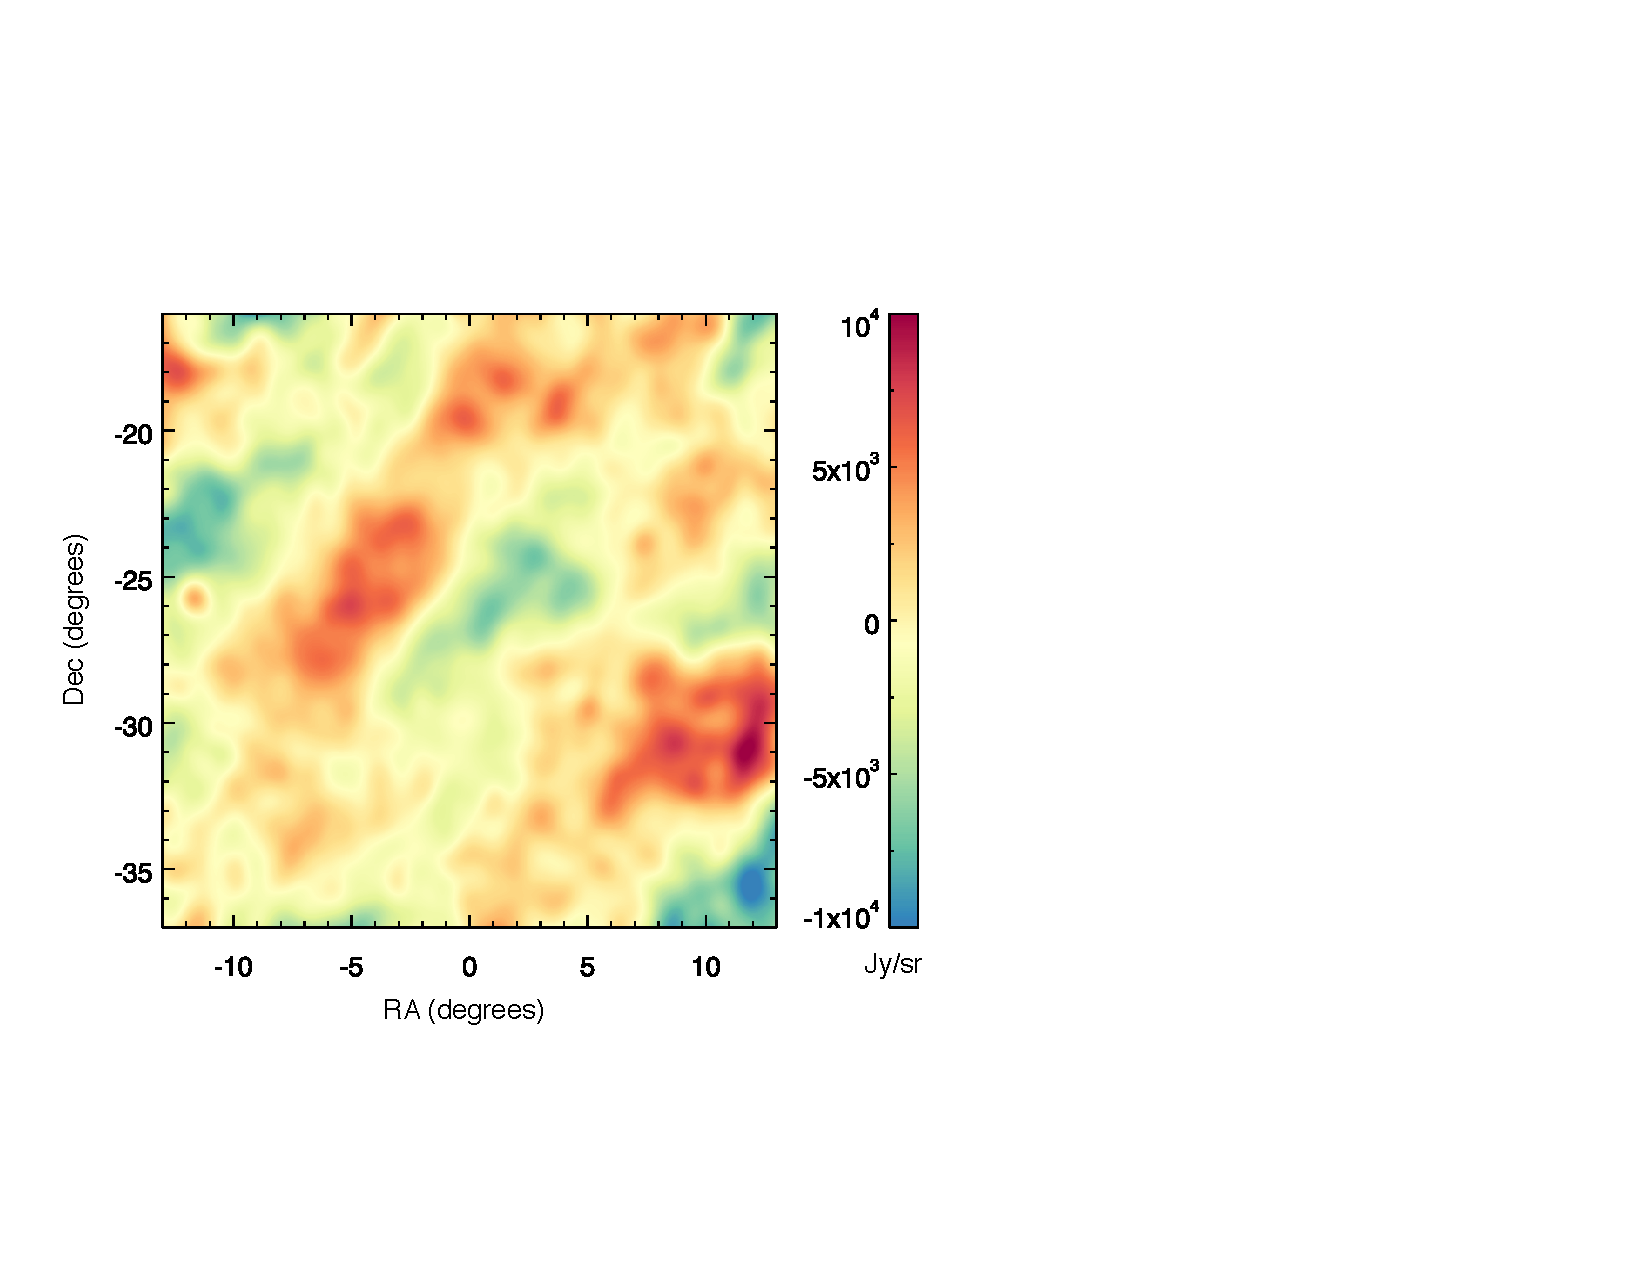
\includegraphics[width=\columnwidth]{diffuse_sky.pdf}
\caption[Diffuse model used for subtraction]{
The diffuse foreground model within the EoR0 field used for foreground subtraction. This 
model was created using residual images from the golden data set. The image shown is 
smoothed to degree scales to emphasize the large scale structure and approximate an 
MWA snapshot natural weighting. The color scale is in units of Jy/str.
\label{fig:diffuse}
}
\end{center}
\end{figure}

We demonstrate the impact of our diffuse model again by running the golden data set 
through our entire analysis pipeline with and without using the diffuse model. Because the 
foreground models used for calibration in the two runs are identical (diffuse is omitted for 
calibration), the calibration solutions were identical and therefore the dirty power spectra 
were identical as well. We compare the model and residual power spectra by direct 
subtraction in Figure~\ref{fig:diffuse_diff}. The top panel shows the model power with the 
diffuse subtracted from the model power without. The entire plot is negative (red) because 
we only added power with the diffuse model. The bottom panel is the difference in residual 
power. The wedge is completely positive (blue), indicating that the diffuse model 
successfully subtracted from the dirty visibilities. The differences in the window are positive 
and negative, indicating that any differences are below the three hour noise level.  

\begin{figure}
\begin{center}
\subfigure{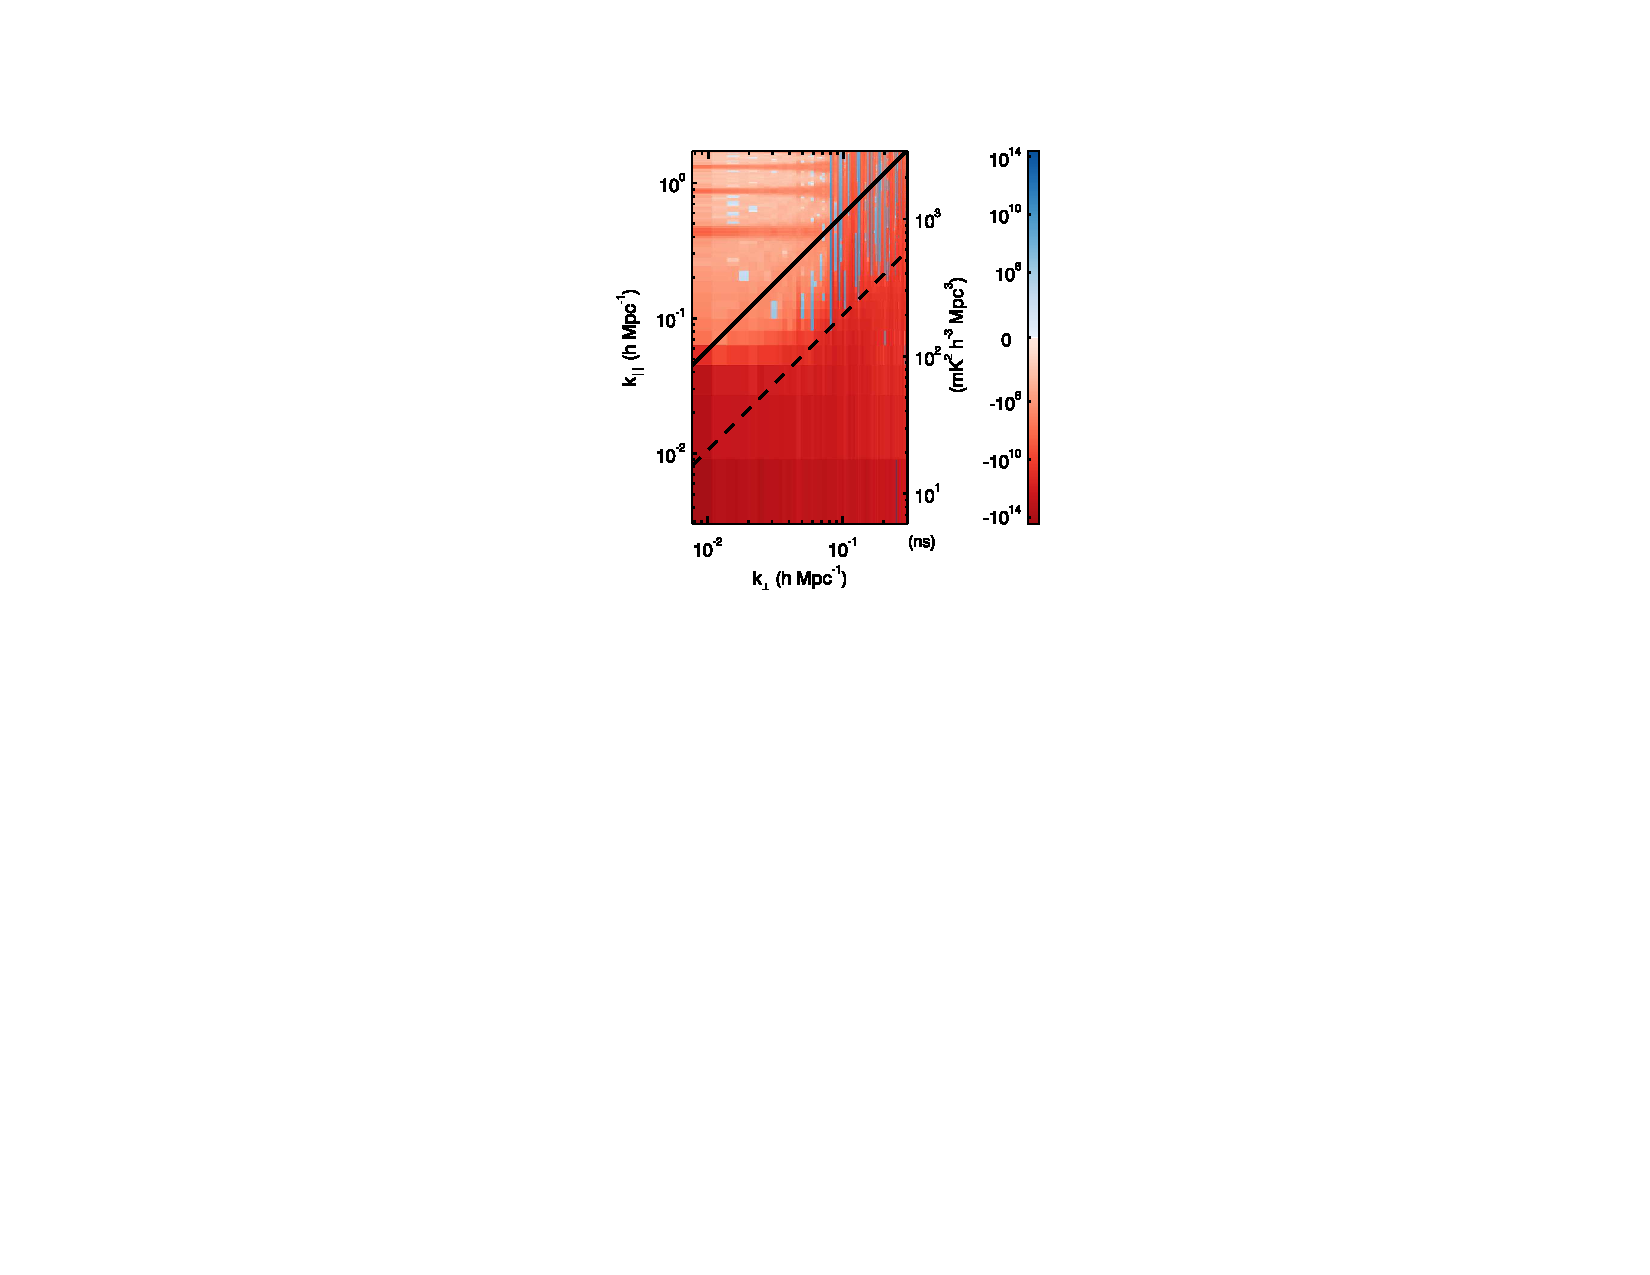
\includegraphics[width=.9\columnwidth]{diffuse_diff_model.pdf}}
~
\subfigure{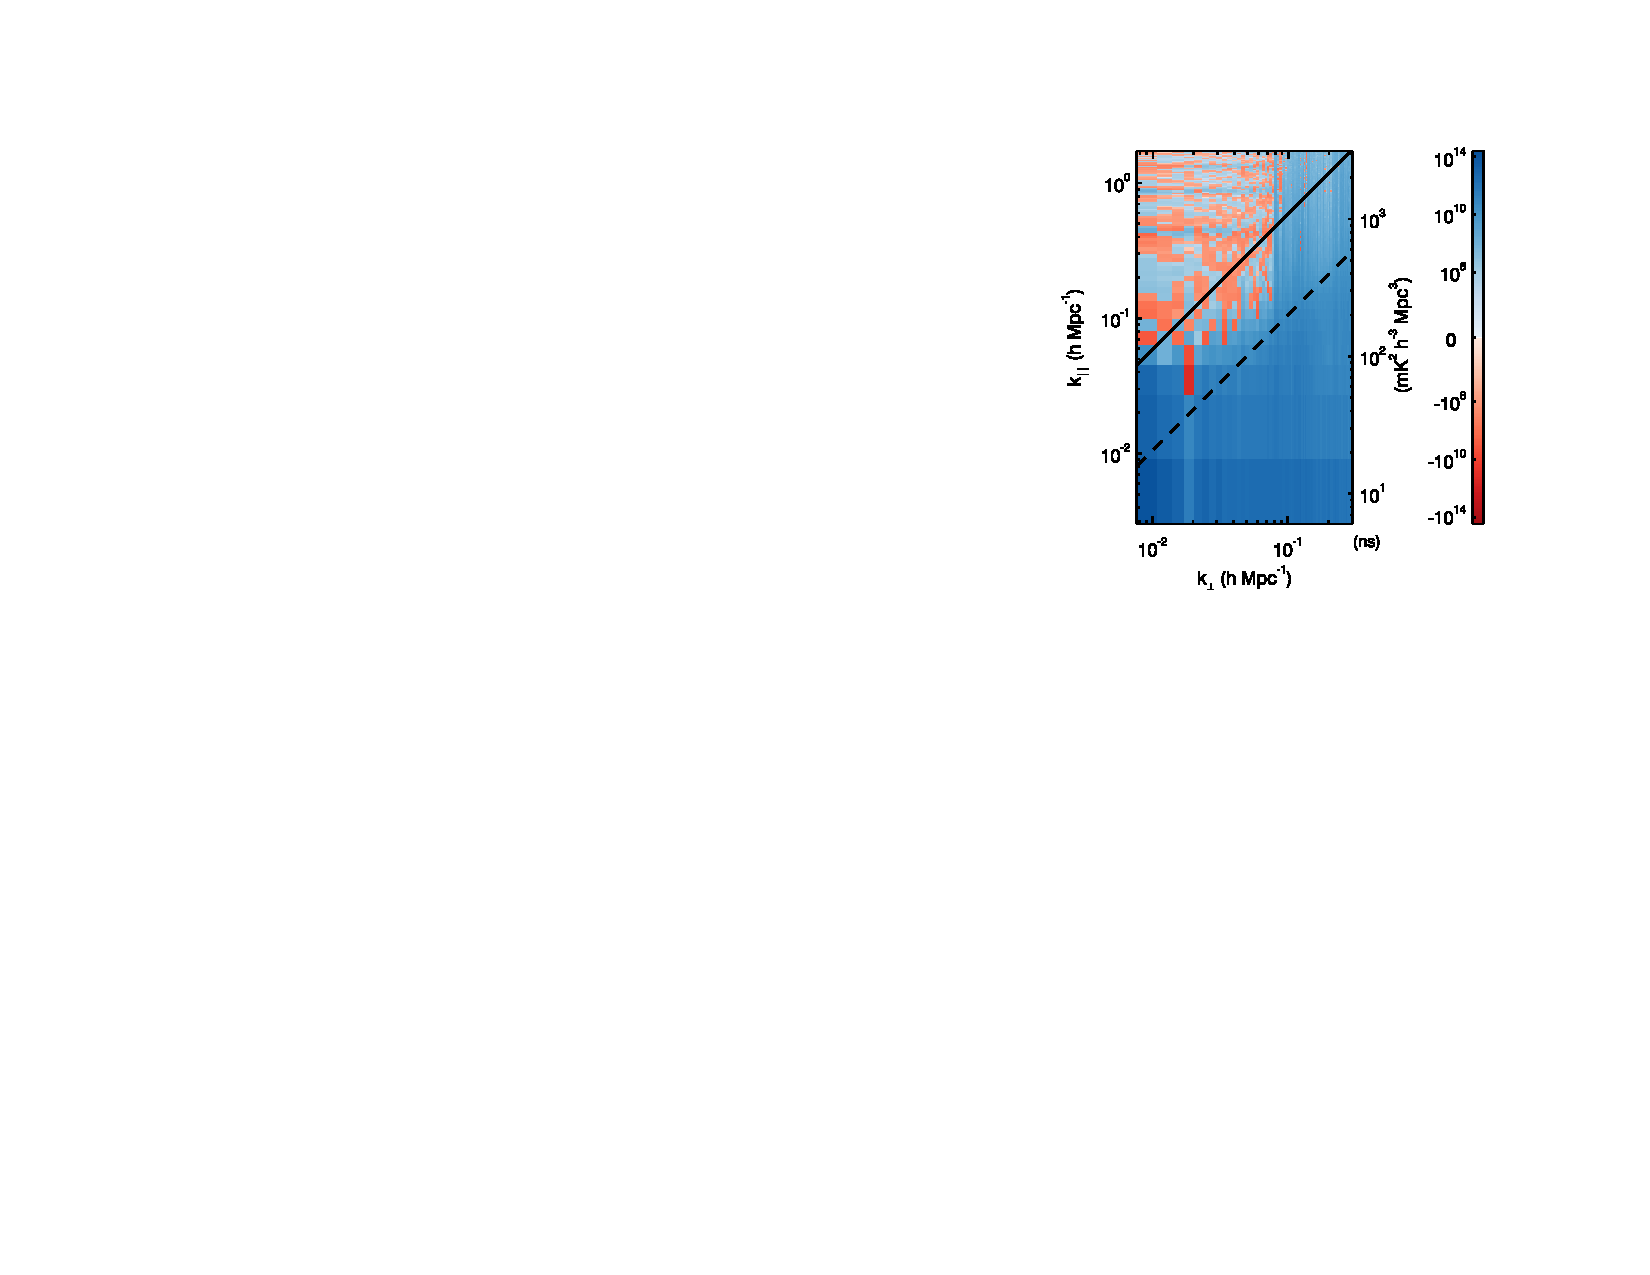
\includegraphics[width=.9\columnwidth]{diffuse_diff_residual.pdf}}
\caption{
Single polarization (E-W) power spectrum differences from the golden data set showing the 
effect of subtracting a diffuse foreground model. The calibration is identical with and without 
the diffuse model, so the dirty power spectra are identical. The diffuse model adds a large 
amount of power to the model (top), and the residual power (bottom) is significantly lower in 
the wedge when using the diffuse model (positive difference), demonstrating a successful 
subtraction. While this first attempt at a diffuse model was rudimentary, it shows promise as 
it successfully removed 90\% of the residual power. 
\label{fig:diffuse_diff}
}
\end{center}
\end{figure}

\section{A Deep Integration}\label{sec:deep}
Up to this point we have only discussed testing and analysis on the three hour golden data 
set. We next turn towards a deep integration, incorporating the techniques described above. 
We start with all MWA observations taken on the EoR0 field at 182~MHz between August 
23, 2013 and November 29, 2013. This includes 2,780 snapshots, or about 86.5 hours of 
data. We first make data quality cuts, then form power spectra.

\subsection{Data Selection}\label{sec:selection}
All 2,780 snapshots in the data set are preprocessed, calibrated, and imaged using the 
pipeline described in the previous sections of this article. Similar to tests on the golden data 
set, we rely heavily on the 2D power spectrum as a diagnostic tool, this time to identify and 
excise poor quality data.

We use the jackknife method -- dividing the data into many subgroups -- to filter out bad 
data and detect patterns. A powerful grouping is to divide the data into the observation day 
and ``pointing" (which direction the antennas were pointed while tracking the EoR0 field). 
We show an example of one day's worth of per-pointing power spectra in Figure~
\ref{fig:jackknife}. The pointings are labeled sequentially with $-5$ corresponding to five 
pointing steps prior to zenith transit, $0$ corresponding to zenith, and $+4$ corresponding 
to four steps after zenith. Early in the night ($-5$ through $-3$) the bulk of the galactic plane 
was still above the horizon, and despite being very far from our primary field of view, highly 
contaminated our observations through the sidelobes of the instrument. We then have 
relatively well behaved pointings, with the EoR window dominated by noise, until the final 
pointing of the night when we can see evidence of the galaxy rising again indicated by 
strong lines of power at the edge of the foreground wedge. We saw the same contamination 
on all days of observation and decided to cut all $-5$, $-4$, $-3$, and $+4$ pointings from 
our data set. In principle it may be possible to model the galactic disk well enough to 
account for its presence, but with a lack of sufficient galactic model, beam model, and the 
analysis tools to include it, we leave this to future work.

\begin{figure*}
\begin{center}
\includegraphics[width=\textwidth]{jackknife.pdf}
\caption[Per pointing jackknife]{An example jackknife test. For this test we divided the data 
into days and pointings. This is an example array of power spectra (residual E-W 
polarization) for a single day, August 26, 2013. The early pointings are heavily contaminated 
by the galaxy in the sidelobes, the window becomes more clear near zenith, and we can 
see trace contamination at the end of the night (pointing +4) when the galaxy has risen 
again.
\label{fig:jackknife}
}
\end{center}
\end{figure*}

Motivated by the hand grading done with power spectrum jackknives, we developed 
another metric to quickly predict power spectrum quality for each snapshot in our data set. 
We do this by forming a delay spectrum \citep{Parsons:2012b} from the raw, uncalibrated 
visibilities. We then calculate an estimated total EoR window power by integrating the 
power above the horizon line and below the first coarse band line. While we would ideally 
use calibrated visibilities for this metric, we have found that the uncalibrated power is 
strongly correlated to the calibrated power, and the cuts we make below are independent of 
calibration. This is encouraging because future analysis could use this metric before 
processing the snapshots, saving valuable computing resources.

We plot the window power for each snapshot in our data set in Figure~\ref{fig:wedge_cut1}. 
We first note that our conclusion from the jackknife tests is confirmed here -- early pointings 
contain strong contamination and have high window power. We also see many outlier 
snapshots with excess power. Inspecting power spectra from these individual snapshots 
confirmed poor data quality, even after calibration. The cause of these contaminants is yet 
unknown, but could easily be attributed to low-level RFI that was missed by the 
\texttt{AOFLAGGER}, or intermittent hardware failures. To remove the poor data we made 
the cut shown with the black box, keeping only snapshots inside.

\begin{figure}
\begin{center}
\subfigure[]{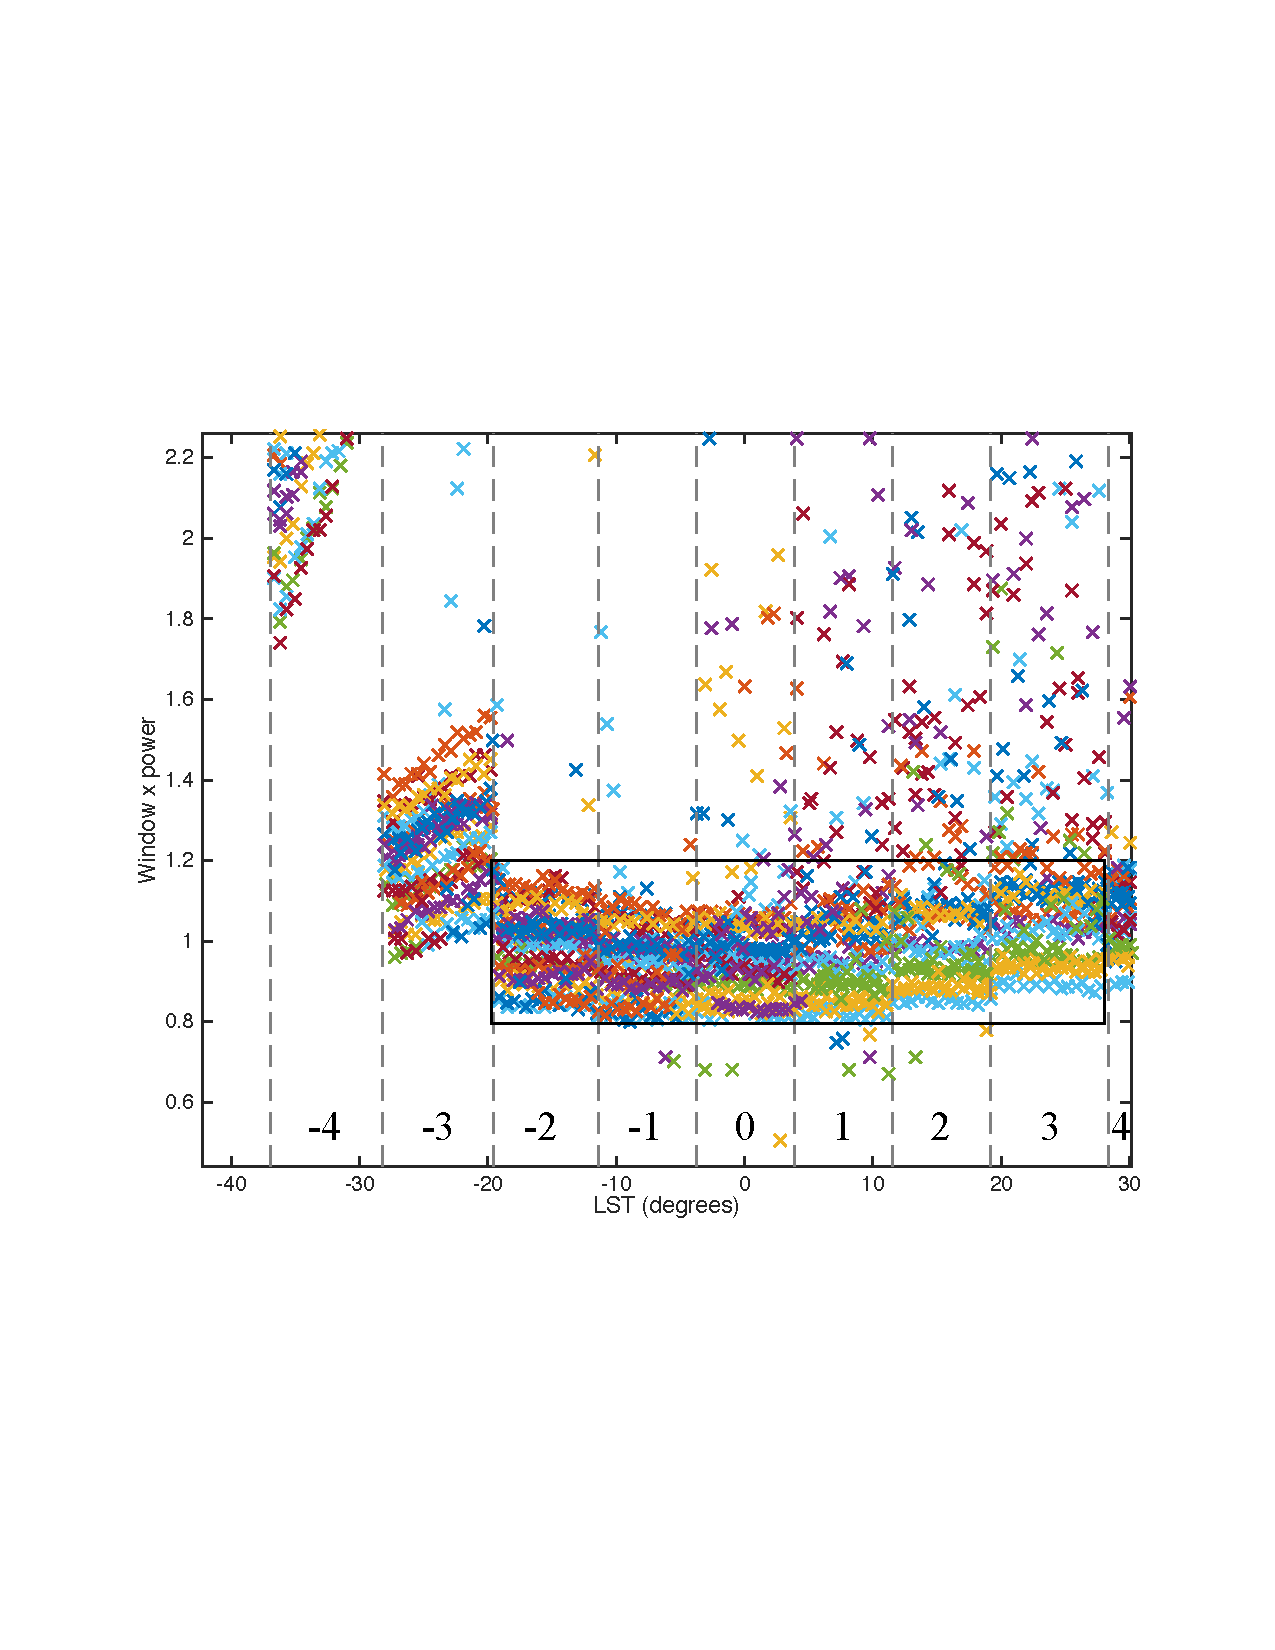
\includegraphics[width=\columnwidth]{window_x_no_cut_box_pointings.pdf}\label{fig:wedge_cut1}}
~
\subfigure[]{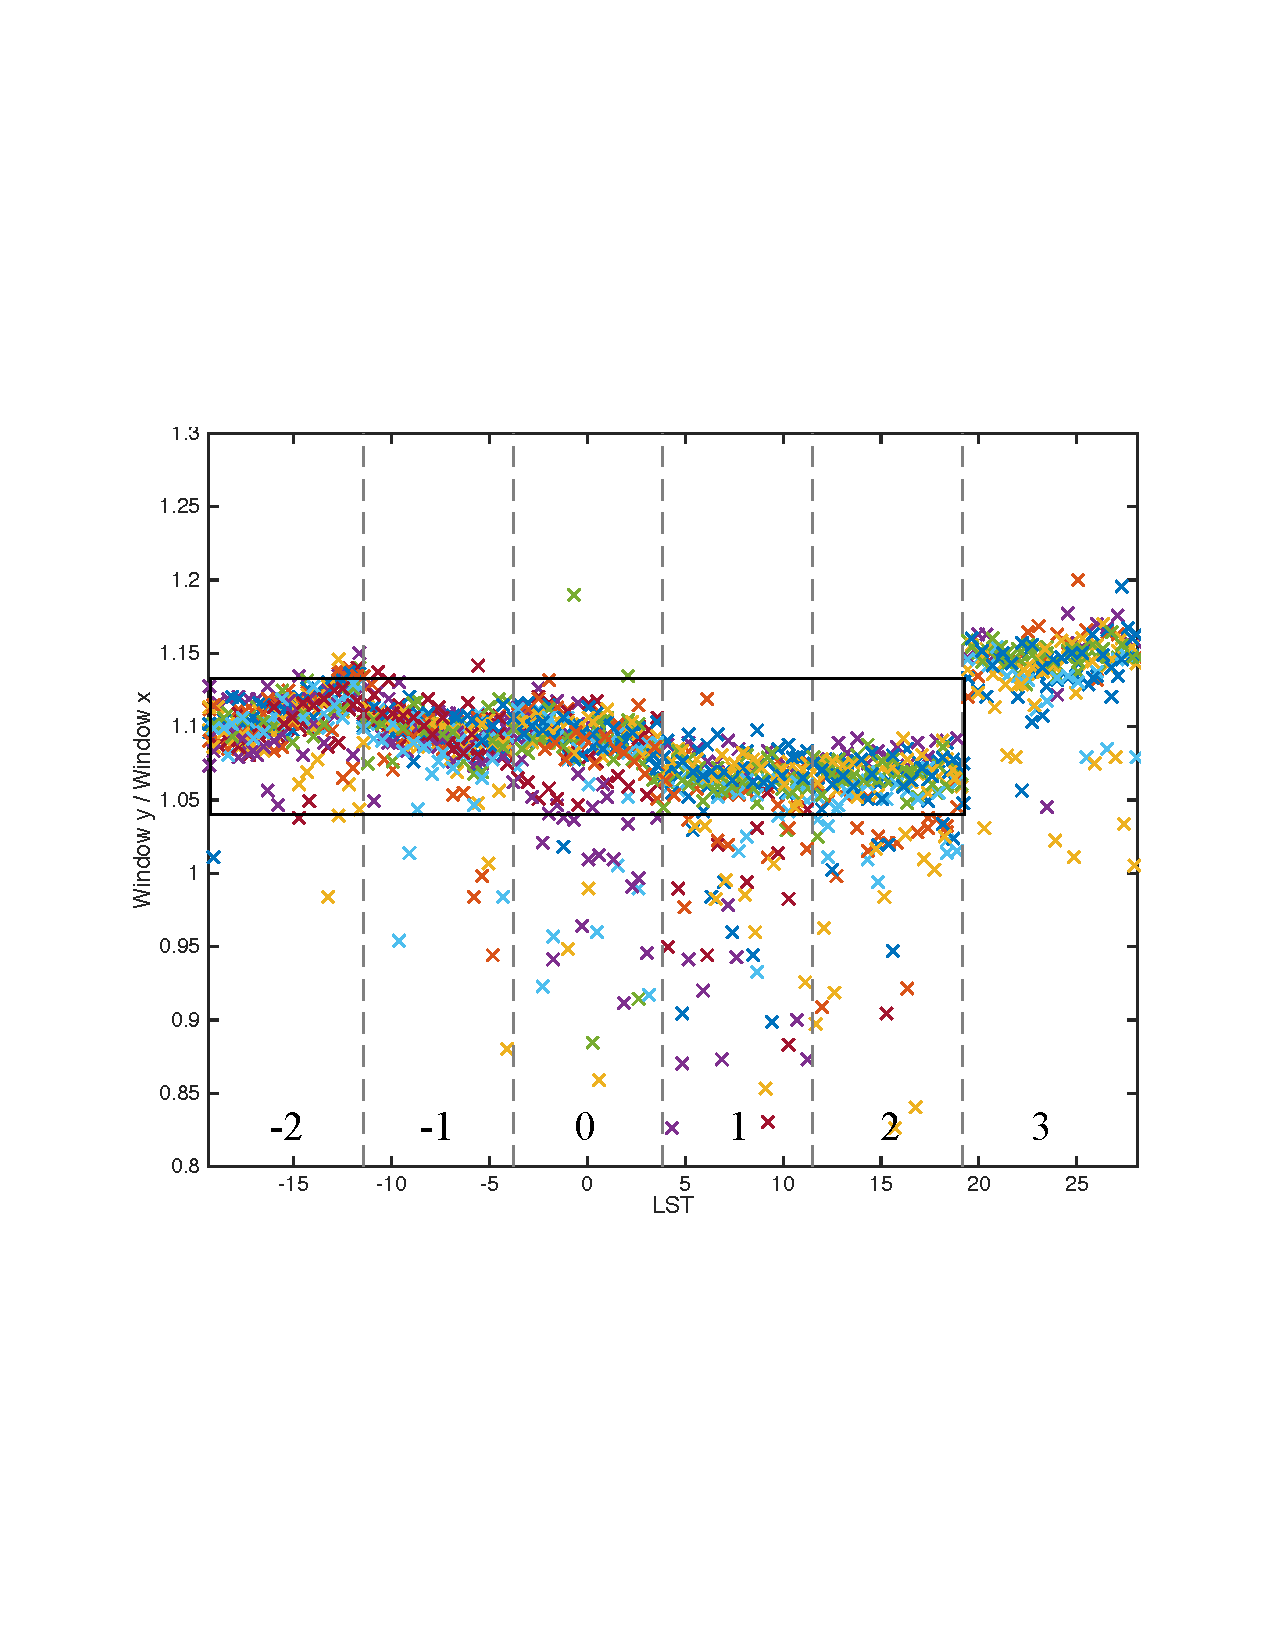
\includegraphics[width=\columnwidth]{window_ratio_cut_v1_box_pointings.pdf}\label{fig:wedge_cut2}}
\caption[Window power cut]{
\emph{Top:} Window power for each observation in our data set. The window power is 
calculated from the delay spectrum of uncalibrated data as a fast quality metric. Each color 
is a distinct day of observing, and the vertical dashed lines represent pointing shifts, with 
the pointing numbers indicated at the bottom of the plot above the horizontal axis. The black 
box indicates observations which passed this cut. \emph{Bottom:} Data cut based on 
window power polarization ratio. For each snapshot that passed the total power cut, we plot 
the ratio of window powers in the N-S and E-W polarizations. Clear outliers can be seen, 
including the whole of pointing +3. The black box again indicates the selected data.
\label{fig:wedge_cut}
}
\end{center}
\end{figure}

Next we compare the power in our two instrumental polarizations. When conducting our 
jackknife tests we saw contamination could exist in one polarization and not the other -- 
potentially due to RFI, or an instrumental failure. We plot the ratio of N-S power to E-W 
power in Figure~\ref{fig:wedge_cut2}, after applying the previous cut. We see the ratio is 
generally flat, with the exception of some outliers and almost all of pointing $+3$. We 
suspect that the excess N-S power in the later pointing is due to the galaxy leaking back 
into the sidelobe of the N-S polarization, but not in the other. Again, we make the cut shown 
with a black box.

Our final data cut was made when inspecting the residual continuum images output from 
FHD. We calculate a fractional residual flux RMS in the following way. For each snapshot 
continuum image, we find the residual flux in the pixels of all sources greater than 0.5 Jy 
subtracted within half-beam power and scale by the integrated flux of the sources. This 
gives us a list of fractional residual fluxes for the snapshot, which we then use to calculate 
an RMS. We found that most snapshots had residual flux RMS $<10\%$ with some outliers, 
which we cut from the data. This cut largely overlapped with previous cuts, but removed an 
additional 95 observations. The cause of the high residual flux RMS is yet unknown and is 
not localized by observation day, LST, pointing, or any other jackknife we have performed.

After the cuts described above, we are left with 1,029 snapshots, or just over 32 hours of 
data. This is an aggressive cut, with the aim of removing all poor quality data and retaining 
a clean data set. As mentioned earlier, more sophisticated analysis could allow us to 
recover data cut from this study in the future (e.g. modeling and removing the galaxy in 
observations pointing far off zenith).

\subsection{Results}\label{sec:results}

In this section we discuss the results after processing the remaining 32~hours of data 
through the \eppsilon pipeline, and place an upper limit on the EoR power spectrum.

The bandwidth of the MWA and our data set is 30.72 MHz, but in order to avoid the effects 
of cosmic evolution over the span of our measured redshift range, we limit observations to 
about 8 MHz, or $\Delta z \sim 0.4$ at our frequency. We do this by dividing the band into 
three overlapping sub-bands of 15.36 MHz each, which, after applying the Blackman-Harris 
window function, will result in effective bandwidths of 7.68 MHz. We label these sub-bands 
as ``low" ($z\approx 7.1$), ``mid" ($z\approx 6.8$), and ``high" ($z\approx 6.5$).

The 32 hour integrated residual power spectra for our three sub-bands and both 
instrumental polarizations are shown in Figure~\ref{fig:2d_ps_subband}. A number of 
features can be seen in these spectra. In all cases the foreground wedge is prominent, with 
extra power at large scales (low $k_{\perp}$). This is indication that our diffuse model can 
improve for deeper subtraction. 

\begin{figure*}
\begin{center}
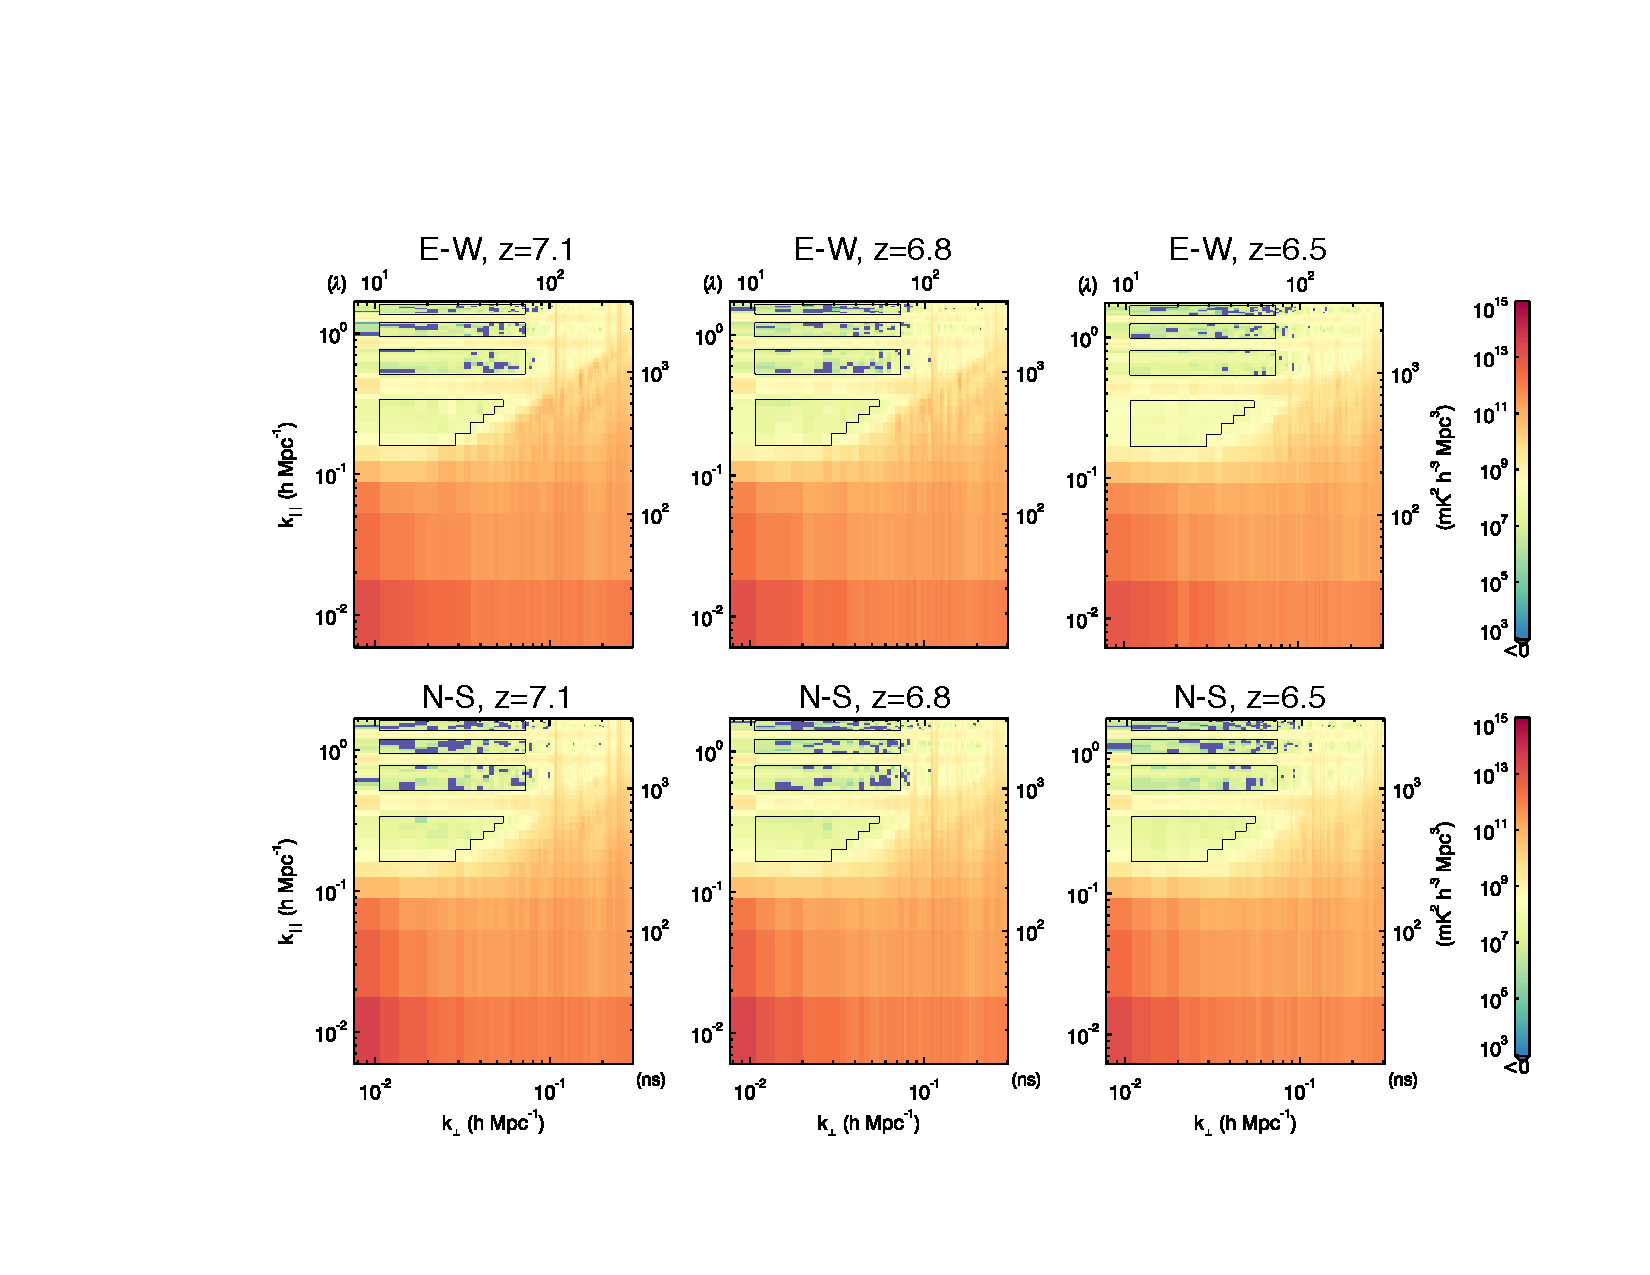
\includegraphics[width=\textwidth]{2d_res.pdf}
\caption[Deep 2D sub-band power spectra]{
Residual two dimensional power spectra for the three sub-bands used to place limits on the 
cosmological signal. The left panels show the low band, centered at 174.7 MHz, or a 
redshift of 7.1. The middle panels show the mid band, centered at 182.4 MHz, or a redshift 
of 6.8. The right panels show the high band, centered at 190.1 MHz, or a redshift of 6.5. 
The red box in the upper left panel shows the window used for averaging to one dimension.
\label{fig:2d_ps_subband}
}
\end{center}
\end{figure*}

The lowest region of the EoR window, above the horizon line and around $k_{||} \approx 
0.25$ h Mpc$^{-1}$, contains purely positive bins, indicating non-noise-like power. The 
cause for this seeming leakage is yet unknown, but will ultimately limit our integration in this 
analysis. One suspected origin of this contamination was individual snapshots with high 
contamination that slipped through our cuts. However, dividing the data into random 
subsets and comparing results indicated that there is not a small number of offending 
observations, instead the leakage appears to exist at a low level in all the data.

Moving up in the window, between the first two coarse band harmonic lines we can see an 
additional faint line. This is the re-emergence of the 150 meter cable reflections. While the 
method described in Section~\ref{subsec:cal_imaging} sufficiently calibrated out this 
reflection line for the three hour golden set integration, the lower noise level in this deeper 
integration shows it is not completely removed. Future analysis will require higher signal-to-
noise on the reflection fitting, which may require combining snapshots for calibration 
solutions. 

Between the coarse band harmonic lines and the reflection line, we do see regions where 
our spectra appear noise-like (positive and negative values). This is encouraging despite 
the leakage at lower $k_{||}$. The red box in the upper left 2D spectrum shows the region of 
$\mathbf{k}$-space we use when averaging to one dimension. We exclude any voxels 
below the solid black horizon line, as well as $k_{||}<0.1$ h Mpc$^{-1}$ due to foreground 
contamination. We limit the $k_{\perp}$ range due to higher power in the coarse bands at 
low $k_{\perp}$, and the poor $uv$ coverage at high $k_{\perp}$, leading to the vertical 
streaks seen on the right side of the 2D spectra. We set our range to be $0.015$ h Mpc
$^{-1} \leq k_{\perp} \leq 0.03$ h Mpc$^{-1}$. This is an aggressive cut, but confidently 
avoids the vertical streaks of leaked power.

One could additionally mask the coarse band harmonic lines when averaging to one 
dimension. However, because $k_{||} \gg k_{\perp}$ within the red box, our spherical shells 
are approximately constant $k_{||}$, so the coarse bands are still isolated in our average. 
We choose to retain them to avoid empty bins, and to help guide the reader when 
comparing the 2D and 1D spectra. While the red box is shown on the 2D plot, the actual 1D 
averaging is done by returning to the full three dimensional power cubes and performing a 
weighted average in shells.

The resulting one dimensional power spectra are shown in Figure~\ref{fig:1d_ps}, where 
the measured power is shown with solid blue, the 1-$\sigma$ noise level is shown with 
dashed red, and the 2-$\sigma$ upper limit for each bin is shown with dashed magenta. 
Where our unbiased estimator is negative, the absolute value is shown, but with a dashed 
green line. For consistency with the literature, we plot our one dimensional power spectra 
as $\Delta^2(k)=k^3P_{21}(k)/(2\pi^2)$, which has units of mK$^2$.

\begin{figure*}
\begin{center}
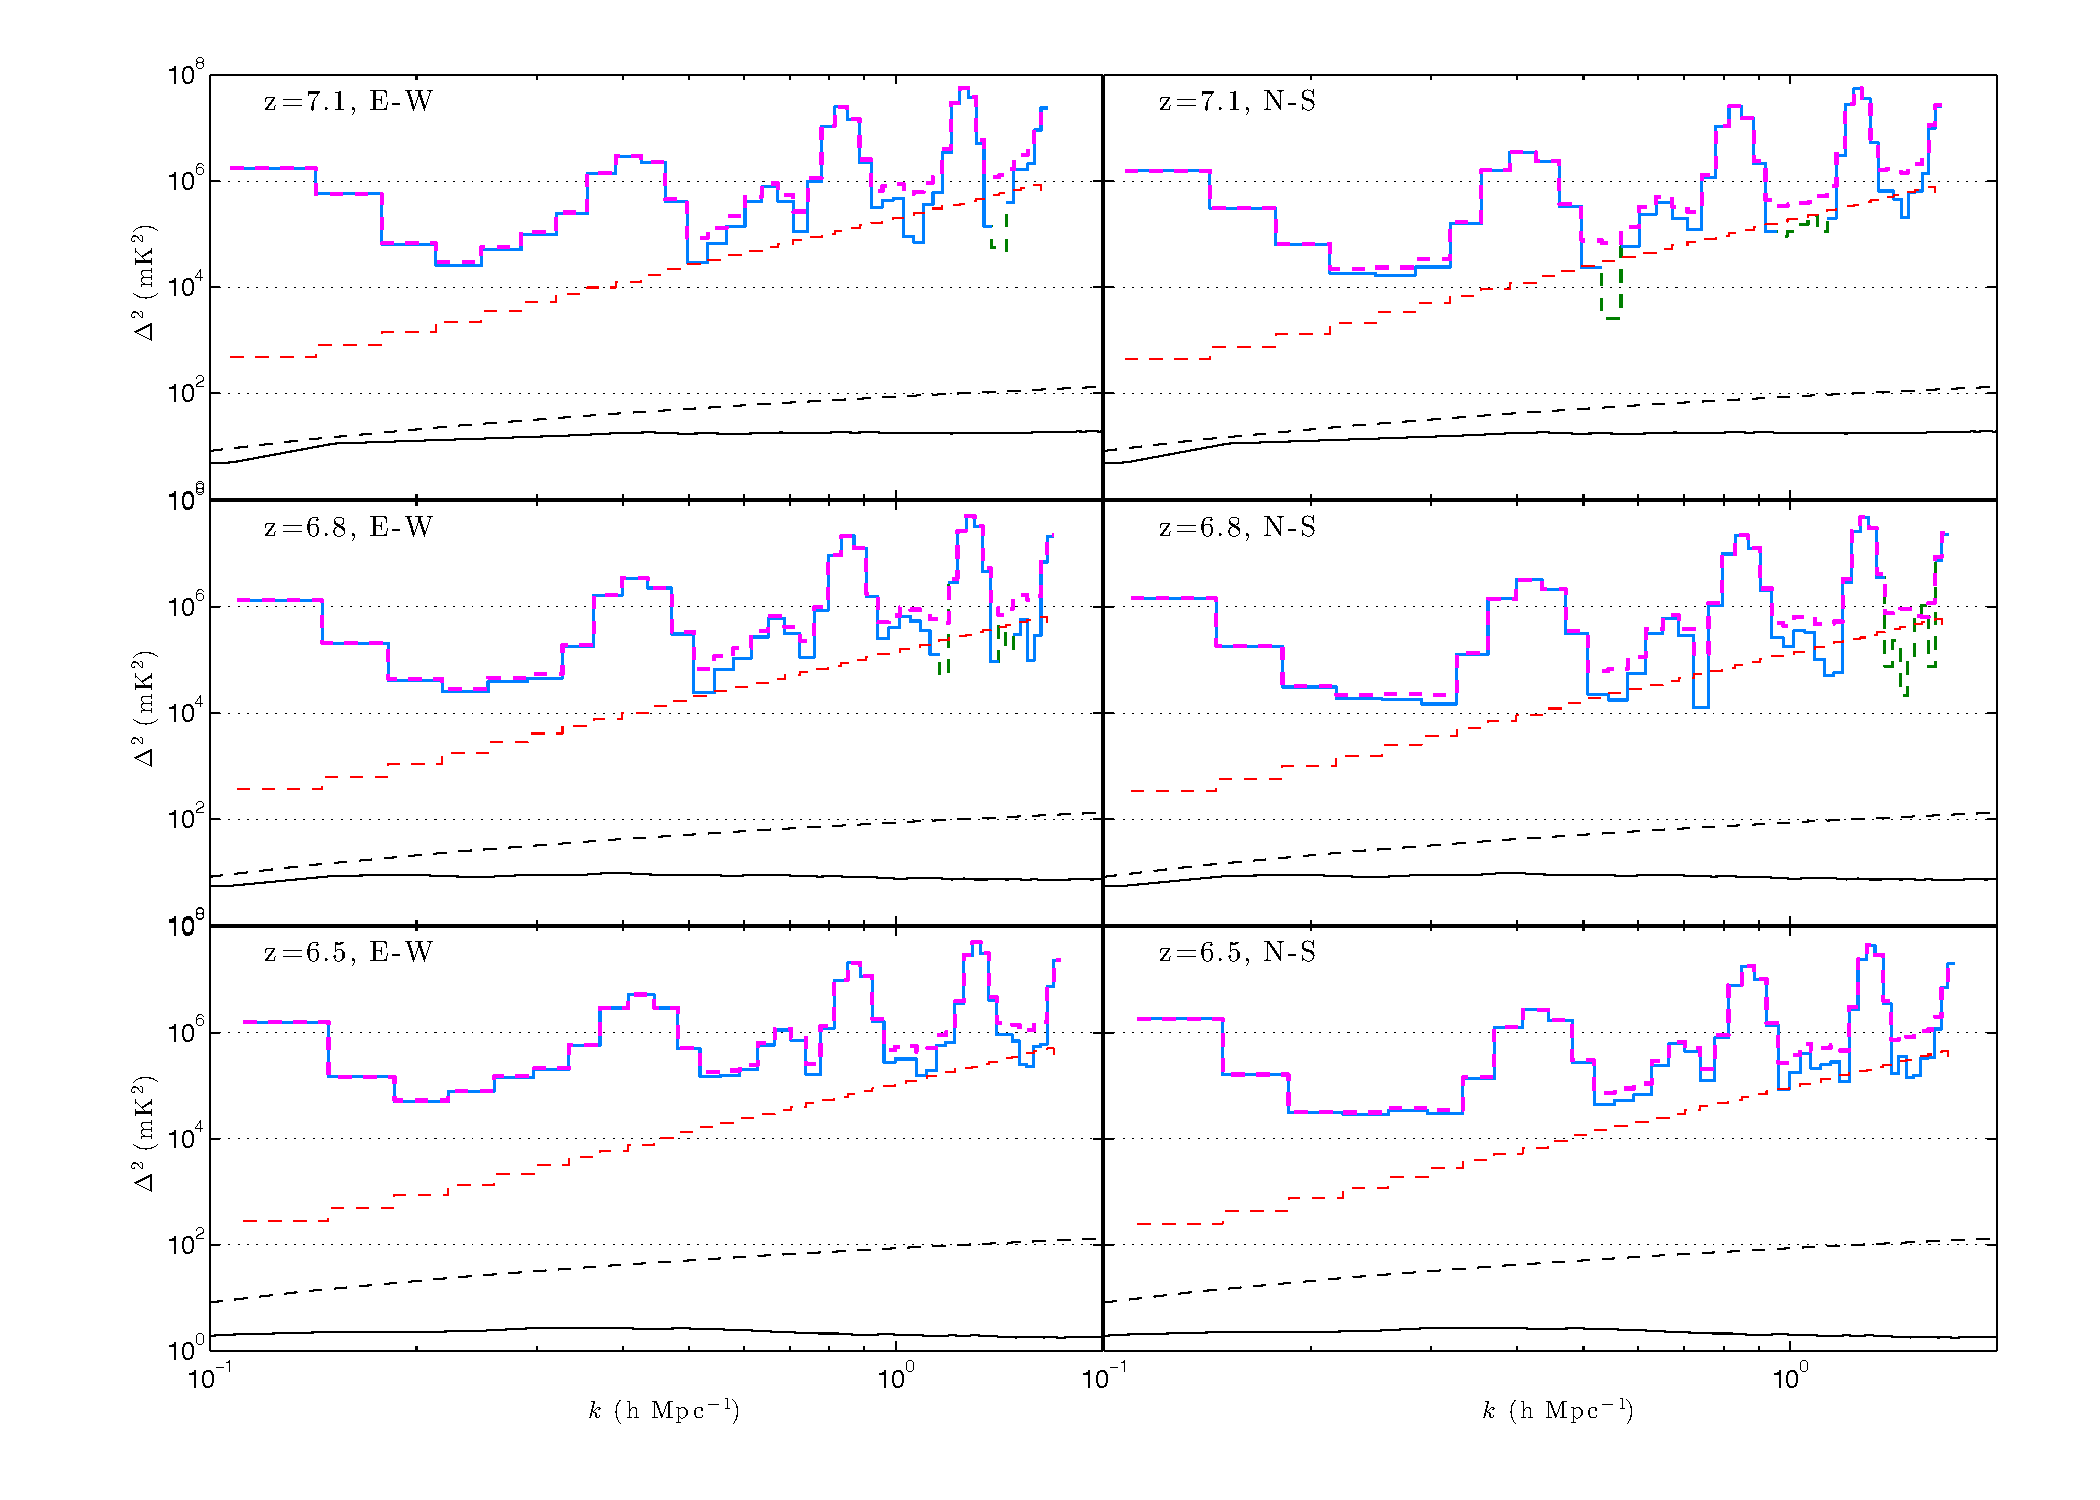
\includegraphics[width=\textwidth]{1D_spectra.pdf}
\caption[1D deep power spectra]{
One dimensional power spectra for our three sub-bands and both instrumental 
polarizations. The solid blue line shows the measured power spectrum with step widths 
corresponding to the bin size used in the average. Where the measured signal is negative 
we plot the absolute value in green. The red dashed line is the 1-$\sigma$ noise level, and 
the dashed magenta line is the 2-$\sigma$ upper limit for each $k$ bin. Theoretical models 
from \citet{Lidz:2008} for $\overline{x}_i=0.54$, $0.82$, and $0.96$ are shown in the low, 
mid, and high band spectra, respectively, in solid black. from \citet{Lidz:2008} are shown in 
solid black. An additional theoretical model for a fully neutral IGM from 
\citet{Furlanetto:2006} is shown with a dashed black line.
\label{fig:1d_ps}
}
\end{center}
\end{figure*}

In all bands and polarizations, we are heavily signal dominated in our most sensitive region 
(low $k$). This is not surprising based on the 2D spectra we examined earlier. We can see 
the strong coarse band harmonic lines, and the cable reflection line between the first two 
coarse band lines. But between these coarse lines there are bins which approach the noise 
level and are consistent with zero (notably the North-South polarization for the $z=7.1$ and 
$z=6.8$ bands). These regions are encouraging because they have the potential to 
continue integrating down with more data.

However, our best upper limits for a cosmological signal are still at low $k$, despite the 
strong leakage. Because any foreground leakage should not correlate with the EoR signal, 
we can assume that the power of the sum of leakage and cosmological signal is greater 
than the power of the EoR signal alone, allowing us to set an upper limit. We quote the best 
2-$\sigma$ upper limits, $\Delta^2_{\text{UL}}$, for each polarization and band in Table~
\ref{tbl:limits}. These limits and their context in the field are further discussed in Section~
\ref{sec:discussion}.

\begin{table}
\begin{center}
\caption[EoR power spectrum limits]{Upper limits on the EoR power spectrum for our three 
sub-bands and two polarizations. Upper limits, $\Delta^2_{\text{UL}}$, are at 97.7\% 
confidence level.
\label{tbl:limits}
}
\begin{tabular}{ccccc}
\tableline\tableline
Sub-band & $z_0$ & Polarization & $k$ (h Mpc$^{-1}$) & $\Delta^2_{\text{UL}}$ (mK$^2$) \\
\tableline
Low & 7.1 & E-W & 0.231 & 3.02 $\times 10^4$\\
Low & 7.1 & N-S & 0.231 & 2.22 $\times 10^4$\\
Mid & 6.8 & E-W & 0.2361 & 2.84 $\times 10^4$\\
Mid & 6.8 & N-S & 0.2361 & 2.17 $\times 10^4$\\
High & 6.5 & E-W & 0.204 & 5.24 $\times 10^4$\\
High & 6.5 & N-S & 0.241 & 3.11 $\times 10^4$\\
\tableline
\end{tabular}
\end{center}
\end{table}

\subsection{Comparison with reference pipeline}\label{subsec:ref_pipe}
\textcolor{red}{Will inject comparison with RTS/CHIPS here.}
% ADAM: Motivation why a pipeline is being discussed
% MAHSA: Summary of RTS to power spectrum (e.g. calibration, etc)
% MAHSA QA: - bad day, forward reference Jordan et al, Beam nulls - fixed for future analysis
% CATH: Plots
%     by pointing - diff zenith vs +2 
%	2D PS vs redshift
%	1D

\section{Discussion}\label{sec:discussion}
Inspecting our 32 hour integrated power spectra we see two places where we are limited. 
First there is a region that is leakage-dominated at low $k$. The cause of this leakage is yet 
unknown, but likely due to imperfect calibration, beam models, and/or foreground models. 
In order to improve on our limit in this regime, future analysis will require calibration which 
better accounts for the instrumental response, perhaps by increasing signal to noise 
through multiple-snapshot solutions or refined antenna response models. Studies of the 
beam are underway \citep[e.g.][]{Neben:2015}, and will likely help to further isolate the 
foreground contaminates in our power spectra. The foreground model is a constant area of 
investigation, but improved spectral dependence in both the point source catalog and the 
diffuse model, as well as the addition of an all-sky galactic model, will continue to improve 
the foreground subtraction and further unlock the EoR window.

The second limited region in our 1D power spectra is between the coarse band harmonics 
where our measured signal approaches the noise level. Additional data will likely reduce the 
noise, and therefore our upper limit, in this regime. However, until the leakage at low $k$ is 
understood, progress at higher $k$ is susceptible to running into the same systematic. 
While a longer integration may improve the upper limit in the short term, the hope for an 
eventual detection lies in understanding the contaminants at low $k$. 

Finally, we place our best upper limits in context with the 21cm EoR field as a whole. A 
direct comparison between measurements from different instruments is difficult due to the 
varying methods, redshifts, and scales probed. However, if we approximate the power 
spectrum in units of mK$^2$ to be roughly flat over the scales probed by the MWA, PAPER, 
and GMRT, we can glean a view of the current state of the field. The results from this 
analysis are a modest improvement over the previous best MWA results \citep{Dillon:2015}, 
which is not surprising given that this integration contains about ten times more data, but 
has a strong signal to noise on the power spectrum. Our results are also consistent with the 
GMRT limit of $\Delta^2\le6.15\times10^4$~mK$^2$ at $z=8.6$ \citep{Paciga:2013}, though 
probe significantly different periods of the EoR. The frontrunner in terms of an upper limit is 
the PAPER experiment \citep{Ali:2015, Jacobs:2015, Parsons:2014}. The PAPER-64 limit of 
$\Delta^2\le502$~mK$^2$ at $z=8.4$ is about one and a half orders of magnitude lower 
than our best limit in power units, though again probing a significantly different redshift. 
While the MWA analysis is not yet at that level of maturity, there is room for rapid 
improvement. The dashed red line in Figure~\ref{fig:1d_ps} indicate the noise level possible 
to reach with this data set if systematics can be overcome.

While this analysis has not reached full potential, it represents the deepest power spectrum 
integration to date produced by an imaging pipeline. Imaging involves many difficulties (e.g. 
efficient gridding and mapmaking, foreground modeling), but if systematics can be 
overcome, it has the potential to quickly compete with other more pointed experiments and 
analysis styles. Here we have identified a crucial region of power spectrum space that is 
currently contaminated, with suggestions for improvement in future analysis. With improved 
calibration techniques, primary beam models, and understanding of foregrounds, the MWA 
and other imaging analyses will be able to quickly approach the most competitive upper 
limits in the field.

\section{Acknowledgements}
This work was supported by NSF grants AST-1410484 and AST-1206552.
JCP is supported by an NSF Astronomy and Astrophysics Fellowship under award 
AST-1302774. This scientific work makes use of the Murchison Radio-astronomy 
Observatory, operated by CSIRO. We acknowledge the Wajarri Yamatji people as the 
traditional owners of the Observatory site. Support for the MWA comes from the U.S. 
National Science Foundation (grants AST-0457585, PHY-0835713, CAREER-0847753, and 
AST-0908884), the Australian Research Council (LIEF grants LE0775621 and LE0882938), 
the U.S. Air Force Office of Scientific Research (grant FA9550-0510247), and the Centre for 
All-sky Astrophysics (an Australian Research Council Centre of Excellence funded by grant 
CE110001020). Support is also provided by the Smithsonian Astrophysical Observatory, the 
MIT School of Science, the Raman Research Institute, the Australian National University, 
and the Victoria University of Wellington (via grant MED-E1799 from the New Zealand 
Ministry of Economic Development and an IBM Shared University Research Grant). The 
Australian Federal government provides additional support via the Commonwealth Scientific 
and Industrial Research Organisation (CSIRO), National Collaborative Research 
Infrastructure Strategy, Education Investment Fund, and the Australia India Strategic 
Research Fund, and Astronomy Australia Limited, under contract to Curtin University. We 
acknowledge the iVEC Petabyte Data Store, the Initiative in Innovative Computing and the 
CUDA Center for Excellence sponsored by NVIDIA at Harvard University, and the 
International Centre for Radio Astronomy Research (ICRAR), a Joint Venture of Curtin 
University and The University of Western Australia, funded by the Western Australian State 
government.

\bibliography{bib}

\end{document}
